% This file was converted to LaTeX by Writer2LaTeX ver. 1.6.1
% see http://writer2latex.sourceforge.net for more info
\documentclass[a4paper,12pt,dvipdfmx]{jarticle}
\usepackage[utf8]{inputenc}
\usepackage{amsmath}
\usepackage{amssymb,amsfonts,textcomp}
\usepackage[T1]{fontenc}
\usepackage[english]{babel}
\usepackage{color}
\usepackage{array}
\usepackage{supertabular}
\usepackage{hhline}
\usepackage{wrapfig}
\usepackage{lastpage}
\usepackage{boxedminipage}
\usepackage[dvipdfmx]{hyperref}
\usepackage{pxjahyper}
\usepackage{url}
\hypersetup{colorlinks=true, linkcolor=blue, citecolor=blue, filecolor=blue, urlcolor=blue}
\usepackage[dvipdfmx]{graphicx}
\graphicspath{%
{./text08-img/}%
}

\newcounter{Exercise}
\newcounter{Question}
\renewcommand\theExercise{例題 8-\arabic{Exercise}}
\renewcommand\theQuestion{\textbf{問題 8-\arabic{Question}}}
% Outline numbering
\setcounter{secnumdepth}{3}
\renewcommand\thesection{\arabic{section}}
\renewcommand\thesubsection{\arabic{section}.\arabic{subsection}}
\renewcommand\thesubsubsection{\arabic{section}.\arabic{subsection}.\arabic{subsubsection}}
\makeatletter
\newcommand\arraybslash{\let\\\@arraycr}
\makeatother
% Page layout (geometry)
\setlength\voffset{-1in}
\setlength\hoffset{-1in}
\setlength\topmargin{2cm}
\setlength\oddsidemargin{2cm}
\setlength\textheight{24.770668cm}
\setlength\textwidth{17.006cm}
\setlength\footskip{26.144882pt}
\setlength\headheight{0cm}
\setlength\headsep{0cm}
% Footnote rule
\setlength{\skip\footins}{0.12cm}
\renewcommand\footnoterule{\vspace*{-0.018cm}\setlength\leftskip{0pt}\setlength\rightskip{0pt plus 1fil}\noindent\textcolor{black}{\rule{0.25\columnwidth}{0.018cm}}\vspace*{0.102cm}}
% Pages styles
\makeatletter
\newcommand\ps@Standard{
  \renewcommand\@oddhead{}
  \renewcommand\@evenhead{}
  \renewcommand\@oddfoot{\hfill 子どもIT未来塾 第8回\hfill Page \thepage{} of \pageref{LastPage}}
  \renewcommand\@evenfoot{\@oddfoot}
  \renewcommand\thepage{\arabic{page}}
}
\newcommand\ps@FirstPage{
  \renewcommand\@oddhead{}
  \renewcommand\@evenhead{}
  \renewcommand\@oddfoot{}
  \renewcommand\@evenfoot{\@oddfoot}
  \renewcommand\thepage{\arabic{page}}
}
\makeatother
\pagestyle{Standard}
\setlength\tabcolsep{1mm}
\renewcommand\arraystretch{1.3}
\newcounter{Figure}
\renewcommand\theFigure{\arabic{Figure}}
\title{\Huge\bf\vspace{70mm} 子どもIT未来塾 第8回}
\author{
清水 尚彦 先生}
\date{}
\begin{document}
\clearpage\setcounter{page}{1}\pagestyle{Standard}
\maketitle
\thispagestyle{FirstPage}

\bigskip

\clearpage\section{今回の授業}
\subsection*{目標 : }
\subsubsection*{ウェブページから欲しい情報を取り出す(スクレイピング)について学ぼう}
\subsection*{注意点}
\begin{itemize}
\item
授業の合間のきゅうけいでは、遠くのものをながめたりして目を休めましょう
\item 水分ほきゅうはこまめにしましょう
\item
先生が説明中は先生の話を聞きましょう
\item
わからないことがあったらTAの先生方にすぐ聞きましょう
\end{itemize}
\subsection*{教科書について}
\begin{itemize}
\item
教科書には例題、それに似た問題があります

\begin{itemize}
\item
まずは、例題をよく読みながら試してみましょう
\item そのあと問題を解きましょう
\end{itemize}
\item
例題、問題をクリアしたらシールラリーカードにシールを貼りましょう
\item
授業中にすべての例題、問題をクリアできたらTAの先生にシールラリーカードを見せて、Complete(コンプリート)シールを貰いましょう
\item
授業中に終わらなかった例題、問題は宿題になるので、できるだけ授業中に終わらせましょう
\item
授業中にわからないところがあったらすぐにTAの先生に聞きましょう
\item
家でわからないことがあったら、すぐに質問フォームから質問しましょう。
\end{itemize}

\bigskip


\bigskip

\clearpage\section{ウェブページから情報を取り出す(準備)}
ウェブページから自分の必要な情報のみ取り出す方法を学びます。
まずはプログラムから自動で情報を取り出すのではなく、スクレイピングの仕組みを理解するために、一つずつ手動で行います。



\bigskip

{\bfseries\color[rgb]{1.0,0.2,0.2}
※ 講義では友達のIPアドレスやwebページを使っていますが、個人で勉強する時は自分の    }

{\bfseries\color[rgb]{1.0,0.2,0.2}
   IPアドレスやwebページを使って例題や問題を行ってください。}

手順
\begin{enumerate}

	\item
グループの席を円と考えましょう。左となりの友達を確認します


\bigskip



\begin{center}
  % Unhandled or unsupported graphics:
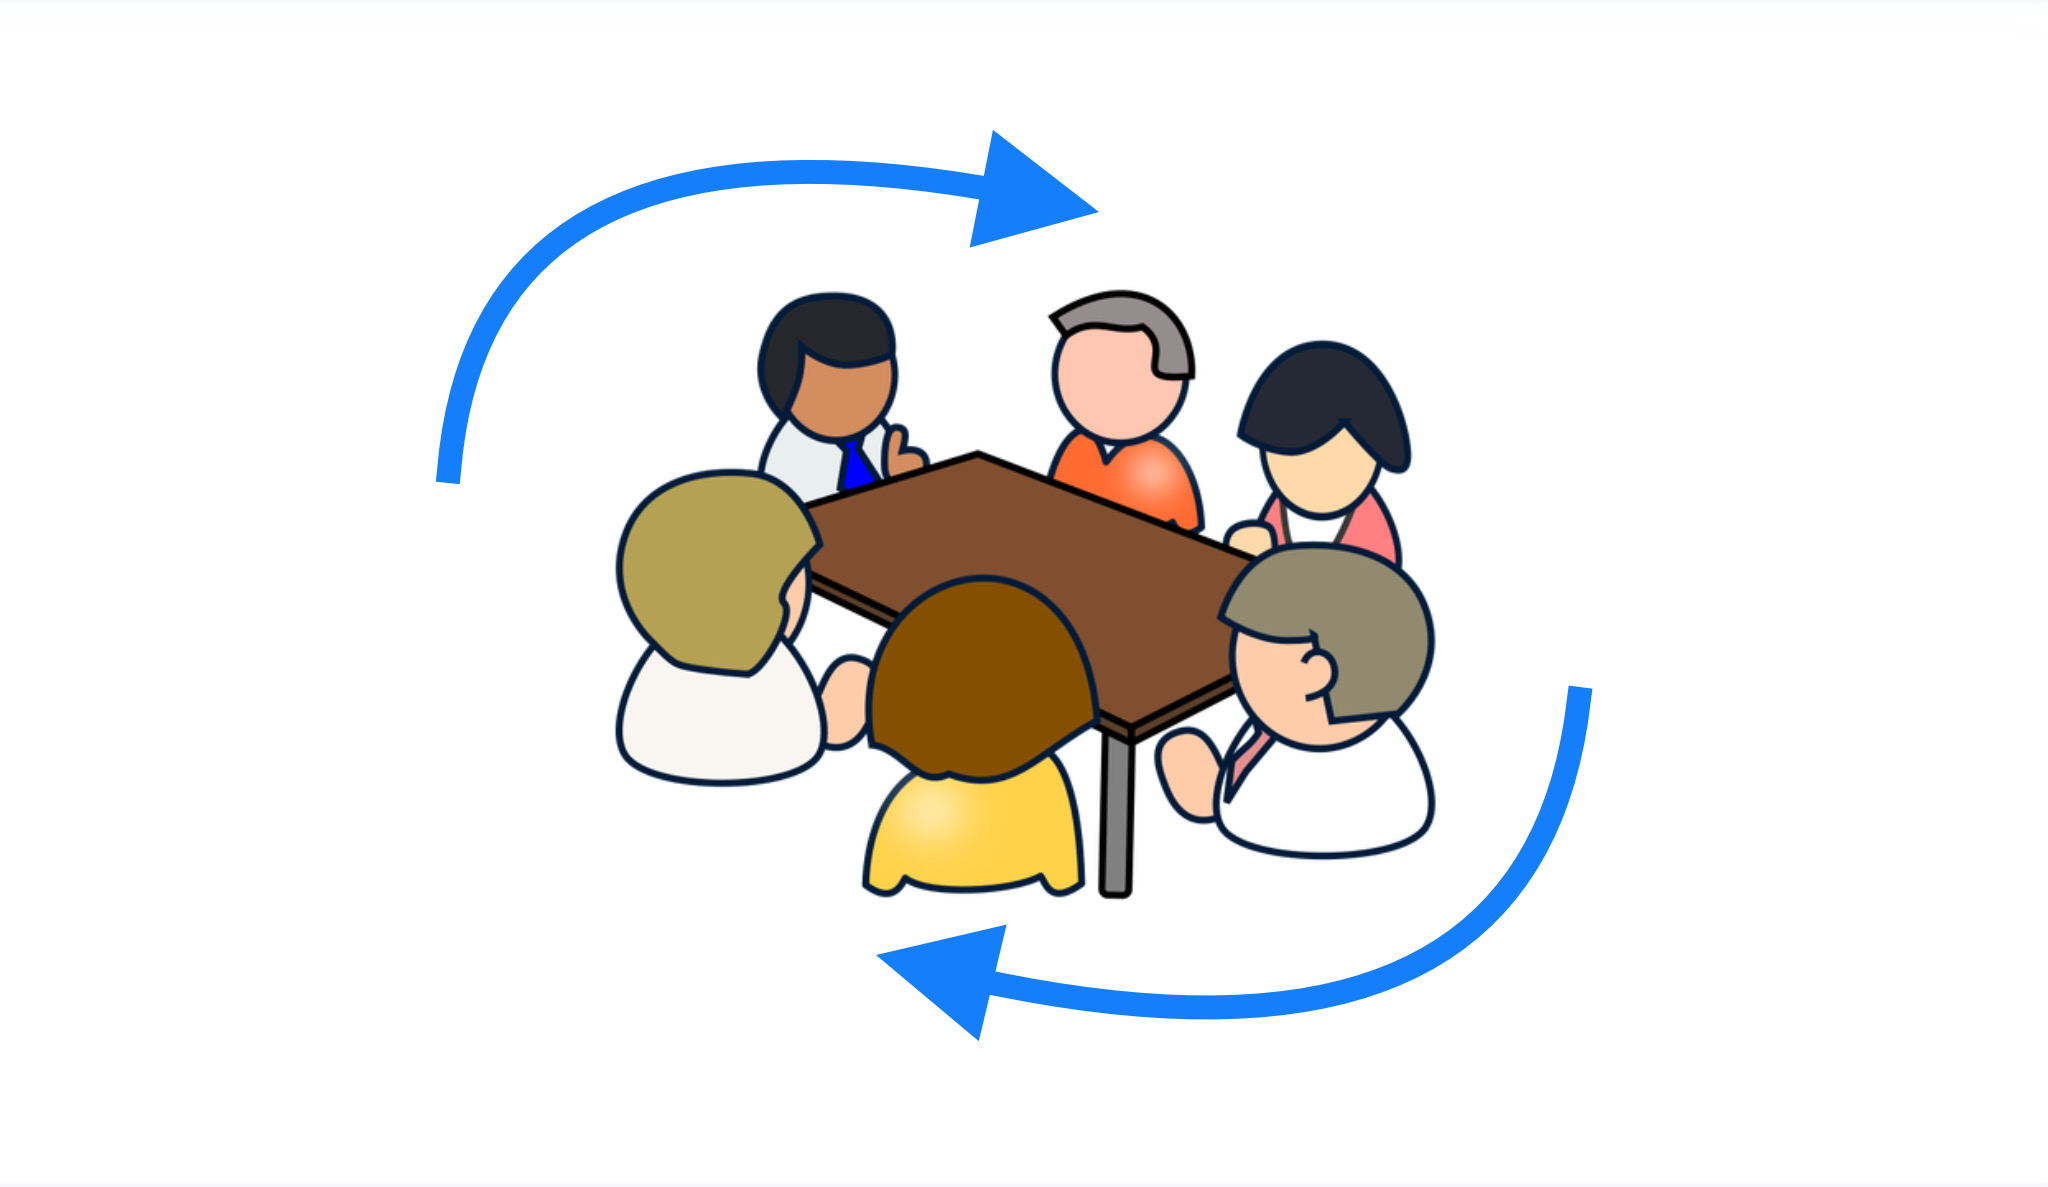
\includegraphics[width=10.174cm,height=5.897cm]{textbook-img001.jpg}

\end{center}

\bigskip


\bigskip


\bigskip



\item
左となりの人の自己紹介ページをダウンロードします

\item
ダウンロードしたページを調べてみましょう。
\end{enumerate}

練習として、左となりの友達のウェブページから情報を取り出します。

そのための準備をしましょう。

1回目に作った自己紹介ページをindex.htmlとしてコピーします

\textbf{cp \ \~{}/01/self\_intro.html \ \ \~{}/08/www/index.html}



\begin{center}
  % Unhandled or unsupported graphics:
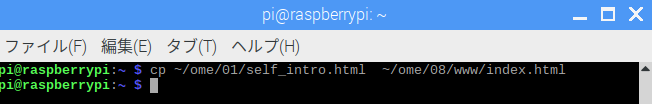
\includegraphics[width=17.006cm,height=3.134cm]{textbook-img002.png}

\end{center}
\clearpage
そのあと、ウェブサーバーを立ち上げます。

ウェブサーバの使い方については「付録 webserver.pyの使い方」を確認してください。

\textbf{cd \ \~{}/08/www}

\textbf{./webserver.py}



\begin{center}
  % Unhandled or unsupported graphics:
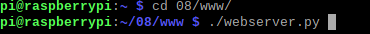
\includegraphics[width=17.006cm,height=2.992cm]{textbook-img003.png}

\end{center}
ウェブサーバーは3000番ポートで動いています。(ポートについては、「7回目の教科書
ポートについて」を確認してください)%
%7会のリファレンス
%koyaman 
%September 23, 2019 10:21 PM


ウェブサーバにアクセスする際は、IPアドレスとともに3000番のポートを指定する必要があります。

このターミナルは閉じずに、もう一つターミナルを開いてください。

\textbf{hostname -I}

を実行して右となりの人にIPアドレスを教えてください。

\begin{center}
  % Unhandled or unsupported graphics:
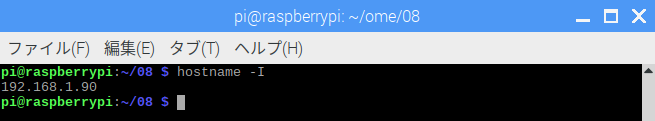
\includegraphics[width=17.171cm,height=3.076cm]{textbook-img004.png}

\end{center}
\clearpage\subsection*{IPアドレスメモらん}
IPアドレスをメモするのに使ってください。

\begin{center}
\tablefirsthead{}
\tablehead{}
\tabletail{}
\tablelasttail{}
\begin{supertabular}{|m{5.4690003cm}|m{5.4690003cm}|m{5.4690003cm}|}
\hline
日付

例: 9/29 &
名前

例: あずまくん &
IPアドレス:ポート

例: 192.168.1.100:3000\\\hline
~

~

~

~
 &
~
 &
~
\\\hline
~

~

~

~
 &
~
 &
~
\\\hline
~

~

~

~
 &
~
 &
~
\\\hline
~

~

~

~
 &
~
 &
~
\\\hline
~

~

~

~
 &
~
 &
~
\\\hline
\end{supertabular}
\end{center}

\bigskip

\refstepcounter{Exercise}
\clearpage\section{\theExercise コマンドラインからウェブページをダウンロードする}
\addtocounter{Exercise}{-1}\refstepcounter{Exercise}\label{E:CURL}
インターネットから情報を取ってくるときに使用するツールは
curl (カール)と言います。 curl
はデータを送ったり受け取ったりするときに使います。

左となりの友達のウェブページを取得してみましょう。

保存するファイル名はローマ字で”友達の名前.html”にしましょう。

例 : koyama.html

例題ではfriend.htmlとして保存しています。

ターミナルを開いてください。

\textbf{cd \ \~{}/08}

curl “左となりの友達のIPアドレス”:3000/index.html -o
friend.html

\ \ 例 :
IPアドレスが192.168.1.90の友達のIPアドレス

\ \ → curl 192.168.1.90:3000/index.html -o friend.html

を実行します。

\begin{center}
  % Unhandled or unsupported graphics:
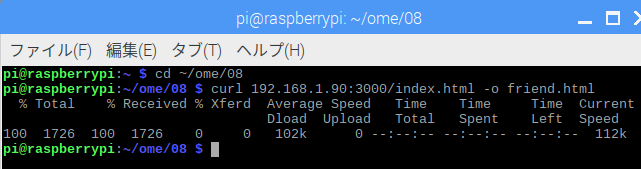
\includegraphics[width=17.006cm,height=4.553cm]{textbook-img005.png}

\end{center}

\bigskip

HTMLファイルをダウンロードしてfriend.htmlとして保存しています。



\begin{center}
\begin{boxedminipage}{17.228cm}
\section*{コラム
curlコマンドのオプション(機能)}

\bigskip

curlコマンドを何もオプションをつけないで実行すると、ターミナルにダウンロードした情報を表示します。コマンドに”-o”オプションをつけることで、ターミナルに表示する代わりに、ファイルに保存することができます。

“-o
“の後に保存するファイル名を指定します。

	\textbf{curl URL -o ファイル名}
\end{boxedminipage}
\end{center}
\clearpage
これでダウンロードができました。実際にダウンロードしたファイルが左となりの友達のウェブページかどうかleafpadで開いて確認してみましょう。



\begin{center}
  % Unhandled or unsupported graphics:
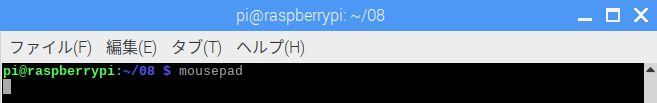
\includegraphics[width=17.006cm,height=2.87cm]{textbook-img006.png}

\end{center}
ファイル(F) → 開く(O).. 

をクリックして\textbf{\~{}/08/friend.html}

を開きます。自己紹介のらんにある名前を探して確認してみよう。



\begin{center}
  % Unhandled or unsupported graphics:
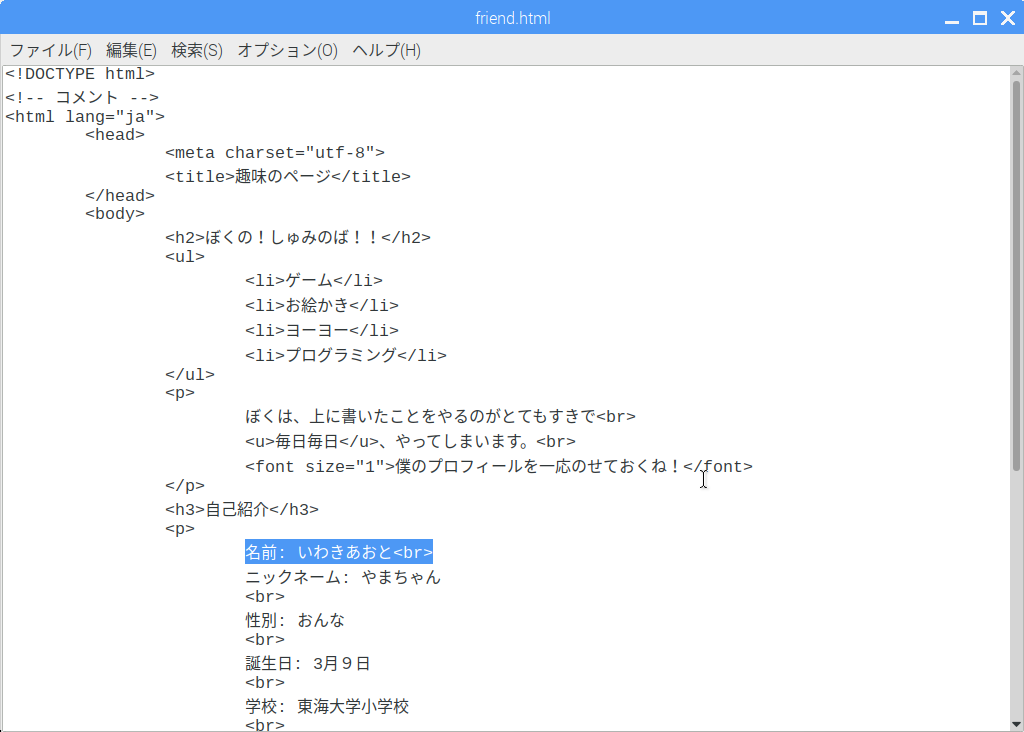
\includegraphics[width=17.006cm,height=12.157cm]{textbook-img007.png}

\end{center}

\bigskip

”いわきあおと”のウェブページのHTMLファイルがダウンロードできていることが確認できました。

次はダウンロードしたHTMLファイルから情報を取り出してみよう。
\refstepcounter{Question}
\clearpage\subsection*{\theQuestion}
\begin{itemize}
\item curl
を使って、グループの友達全員のウェブページを保存しよう。
\end{itemize}
\ \ \ \ Hint :
ローマ字を使って”友達の名前.html”にしておこう

\ \ \ \ (例: koyama.html) 

\refstepcounter{Question}
\subsection*{\theQuestion}
\begin{itemize}
\item
leafpadを使ってダウンロードしたHTMLファイルを開いて友達の名前を確認してみよう
\end{itemize}
\ \ \ \ Hint :
ダウンロードしたファイルをleafpadで見てみよう

\refstepcounter{Exercise}
\clearpage\section{\theExercise ダウンロードしたページを調べてみましょう}
\addtocounter{Exercise}{-1}\refstepcounter{Exercise}\label{E:HTML}
考え方

\ref*{E:CURL}で、友達のウェブページのHTMLをダウンロードしました。次はほしい情報を取り出します。ここでは、テキストエディタで検索をして、ほしい情報を探し抜き出します。

コマンドラインを開いて

\textbf{cd \ \~{}/08/}

leafpad 



\begin{center}
  % Unhandled or unsupported graphics:
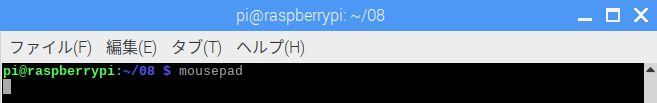
\includegraphics[width=17.006cm,height=2.87cm]{textbook-img006.png}

\end{center}
を実行してください。

テキストエディタが開きます。

ファイル(F) → 開く(O).. 

をクリックして\textbf{\~{}/08/friend.html}



\begin{center}
  % Unhandled or unsupported graphics:
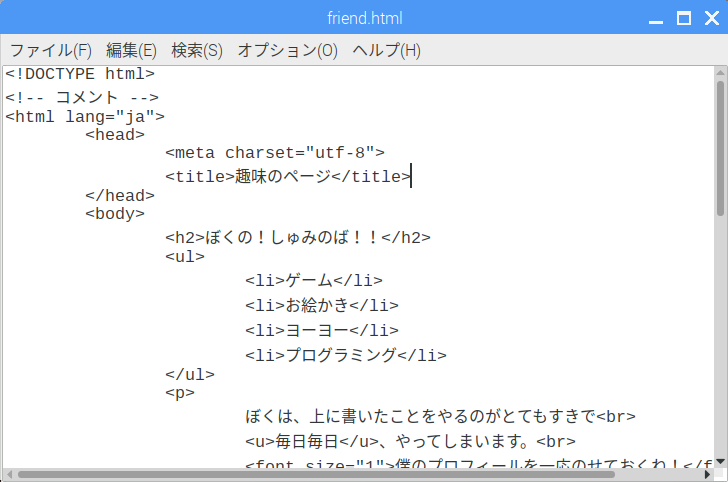
\includegraphics[width=15.074cm,height=9.98cm]{textbook-img008.png}

\end{center}


\bigskip


\bigskip

\clearpage
友達のウェブページのタイトルをテキストエディタで探してみましょう。

タイトルはブラウザのタブに表示されるもので{\textless}title{\textgreater}{\textless}/title{\textgreater}タグで作ったことを思い出しましょう。



\begin{center}
  % Unhandled or unsupported graphics:
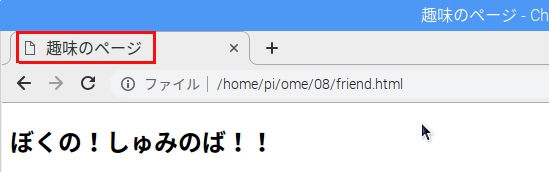
\includegraphics[width=16.782cm,height=5.389cm]{textbook-img009.png}

\end{center}

\bigskip

テキストエディタで{\textless}title{\textgreater}{\textless}/title{\textgreater}タグを探してみましょう。

検索-{\textgreater}検索(F)..をクリックします。

\begin{center}
  % Unhandled or unsupported graphics:
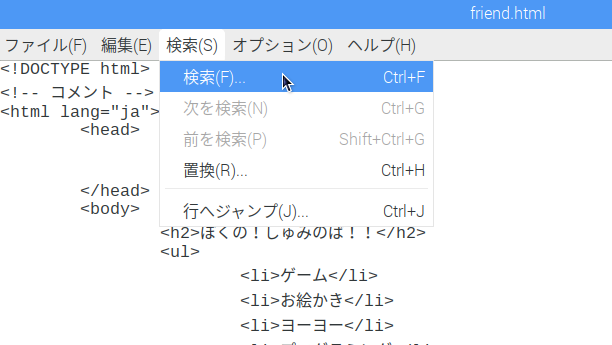
\includegraphics[width=16.533cm,height=7.918cm]{textbook-img010.png}

\end{center}
\clearpage
検索する文字列には検索したい文字列を入れます。この例では{\textless}title{\textgreater}{\textless}/title{\textgreater}を探したいので、

{\textless}title{\textgreater}と入れます。検索をクリックします。

{\bfseries
注意 :
{\textless}title{\textgreater}は半角文字です。入力モードが半角になっているか確認してください。}


\begin{center}
  % Unhandled or unsupported graphics:

\includegraphics[width=16.625cm,height=8.371cm]{textbook-img012.png}

\end{center}
見つかった結果を色を変えて表示してくれます。これで、ウェブページからほしい情報を見つけることができました。


\bigskip

毎回手動で友達のウェブページをダウンロードして、検索して探すのは大変です。次はプログラムから自動で行う方法を学びましょう。
\refstepcounter{Exercise}
\clearpage\section{\theExercise HSPから情報を取り出す}
\addtocounter{Exercise}{-1}\refstepcounter{Exercise}\label{E:SCRAPING}
考え方

前の例題でやったように、毎回手動で友達のウェブページをダウンロードして、テキストエディタを使って検索するのは大変です。
また、ウェブページが更新されたら、同じ手順を繰り返して情報を取り直さないといけません。
そこで、今回はこの手順をHSPのプログラムで自動で行う方法を学びます。

友達のウェブページからウェブページのタイトルを取り出してみよう。

まずはプログラムを動かしてみましょう。

ターミナルからHSPスクリプトエディタを開きます。

ターミナルを開いて、

hsed を実行してください

ファイル→開くから

\begin{center}
  % Unhandled or unsupported graphics:
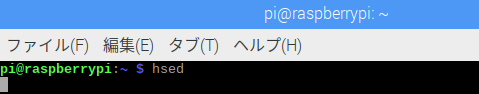
\includegraphics[width=16.94cm,height=2.944cm]{textbook-img013.png}

\end{center}
\textbf{\~{}/08/title.hsp}

を開いてください



\begin{center}
  % Unhandled or unsupported graphics:
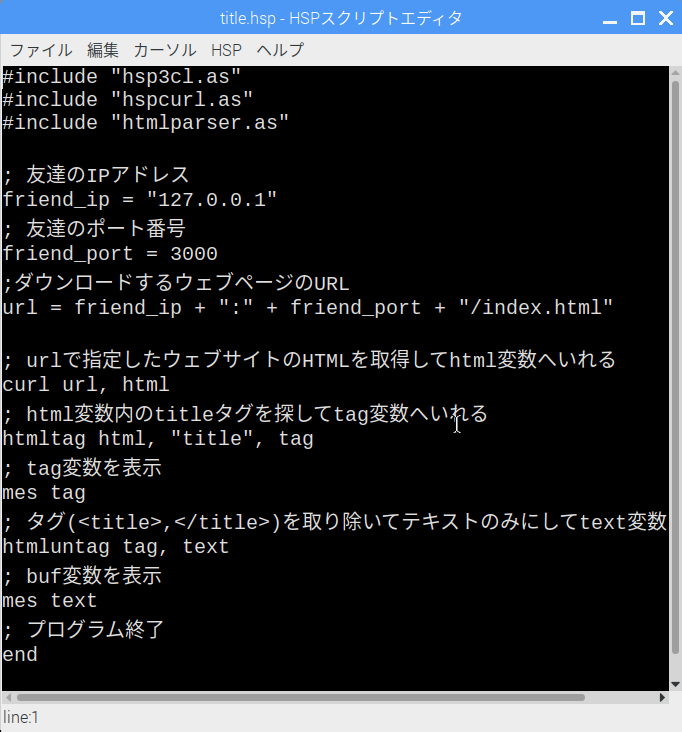
\includegraphics[width=11.472cm,height=12.312cm]{textbook-img014.png}

\end{center}

\bigskip


\bigskip

\clearpage
6行目のfriend\_ip =
“127.0.0.1”を友達のIPアドレスに変えましょう。


例 : 友達のIPアドレスが”192.168.1.90”の場合

\ \ → friend\_ip = “192.168.1.90”

F5を押して実行してみましょう。
実行結果はhsedを実行したターミナルに表示されます。



\begin{center}
  % Unhandled or unsupported graphics:
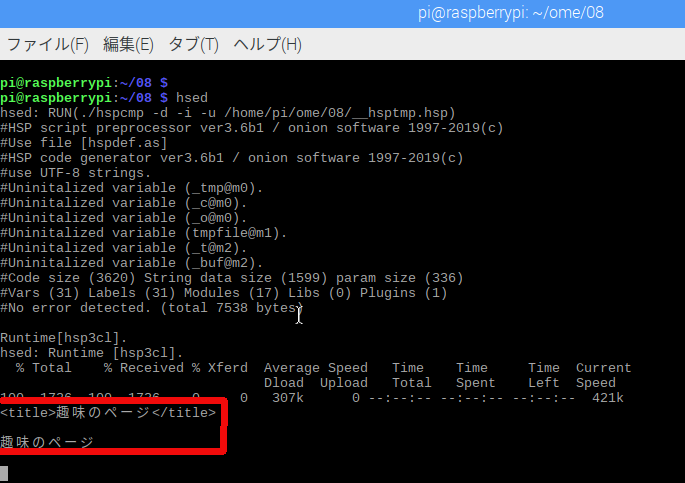
\includegraphics[width=15.411cm,height=11.841cm]{textbook-img015.png}

\end{center}


\bigskip


\bigskip

このように手動でHTMLファイルをダウンロードして、テキストエディタで開いて、タイトルを検索して情報を取り出したのをプログラムで行うことができます。
次にプログラムの中身を見てみましょう。

\clearpage
プログラム解説



\begin{center}
\begin{boxedminipage}{16.053cm}
\setlength{\itemsep}{0cm} % 項目間
\setlength{\parskip}{0cm} % 項目間
\begin{enumerate}
\baselineskip 10pt
\setlength{\itemsep}{0cm} % 項目間
\item \#include {\textquotedbl}hsp3cl.as{\textquotedbl}
\item \#include {\textquotedbl}hspcurl.as{\textquotedbl}
\item \#include {\textquotedbl}htmlparser.as{\textquotedbl}
\item 
\item ; 友達のIPアドレス
\item friend\_ip = {\textquotedbl}127.0.0.1{\textquotedbl}
\item ; 友達のポート番号 
\item friend\_port = 3000
\item ;ダウンロードするウェブページのURL
\item url = friend\_ip + {\textquotedbl}:{\textquotedbl} + friend\_port + {\textquotedbl}/index.html{\textquotedbl}
\item 
\item ;
urlで指定したウェブページのHTMLを取得してhtml変数へいれる
\item curl url, html
\item ;
html変数内のtitleタグを探してtag変数へいれる
\item htmltag html, {\textquotedbl}title{\textquotedbl}, tag
\item ; tag変数を表示
\item mes tag
\item ;
タグ({\textless}title{\textgreater},{\textless}/title{\textgreater})を取り除いてテキストのみにしてtext変数に入れる
\item htmluntag tag, text
\item ; buf変数を表示
\item mes text
\item ; プログラム終了
\item end
\end{enumerate}
\end{boxedminipage}
\end{center}

\bigskip



\bigskip

6行目のfriend\_ip変数にはウェブページをダウンロードする友達のIPアドレスを入れます。

自分のウェブページをダウンロードしたい場合は、”127.0.0.1”を指定します。


\bigskip

8行目のfriend\_port変数にはウェブサーバが動いているポートを指定します。
3000番でウェブサーバが動いているので、3000にしておきます。


\bigskip

10行目のurl変数は、ダウンロードするウェブページを表すURLを指定します。

この例題プログラムでは、127.0.0.1:3000/index.htmlのような形になっています。


\bigskip

13行目では、実際にウェブページをダウンロードしてhtml変数へいれています。

curl url, html

はurl変数で指定されているウェブページをダウンロードしてファイルの中身をhtml変数へ読み込んでいます。


\bigskip

\clearpage
15行目の

htmltag html, “title”, tag

では、html変数にあるHTMLから{\textless}title{\textgreater}{\textless}/title{\textgreater}タグを探して、結果をtag変数へいれています。


\bigskip

\begin{center}
\tablefirsthead{}
\tablehead{}
\tabletail{}
\tablelasttail{}
\begin{supertabular}{|m{16.806cm}|}
\hline
htmltag命令の使い方

\textbf{htmltag} \textbf{もとの変数, “タグ”,
結果を入れる変数}

例: htmltag src, “title”, dest

 src変数からtitleタグを探して、dest変数へ結果を入れる。\\\hline
\end{supertabular}
\end{center}

\bigskip

17行目では、titleタグの検索結果を表示しています。

表示結果では、{\textless}title{\textgreater}趣味のページ{\textless}/title{\textgreater}となっています。

実際に欲しい情報は{\textless}title{\textgreater}{\textless}/title{\textgreater}の間にある文字列つまりこの例では、”趣味のページ”です。



\begin{center}
  % Unhandled or unsupported graphics:
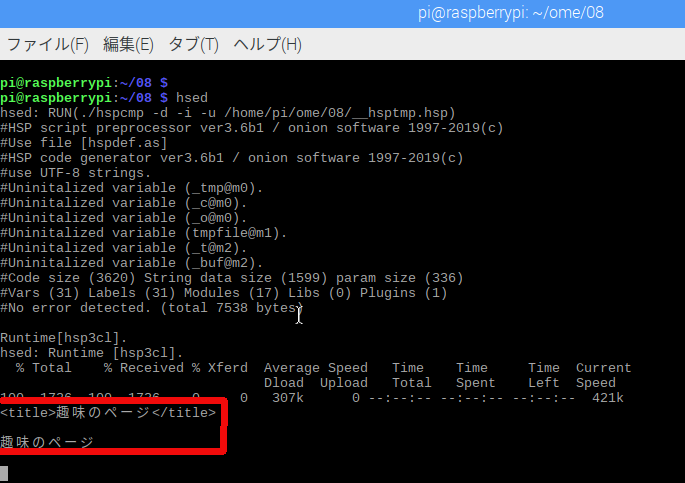
\includegraphics[width=15.411cm,height=11.841cm]{textbook-img015.png}

\end{center}


\bigskip


\bigskip

\clearpage
19行目の

htmluntag tag, text

では、tag変数にあるタグをすべて取り外して、間にあるテキストのみにして、text変数へいれています。


\bigskip

\begin{center}
\tablefirsthead{}
\tablehead{}
\tabletail{}
\tablelasttail{}
\begin{supertabular}{|m{16.806cm}|}
\hline
htmluntag命令の使い方

{\bfseries htmluntag もとの変数, 結果を入れる変数}

例: htmluntag src, dest

src変数のタグを取り外してタグの間にあるテキストだけにしてdest変数へ結果を入れる。\\\hline
\end{supertabular}
\end{center}

\bigskip

21行目では、{\textless}title{\textgreater}{\textless}/title{\textgreater}タグを取り外した結果を表示させています。

タグを取り外したので、{\textless}title{\textgreater}趣味のページ{\textless}/title{\textgreater}の間の文字列である”趣味のページ”のみ表示されています。
ほしいテキストのみを取り出すことができました。



\begin{center}
  % Unhandled or unsupported graphics:
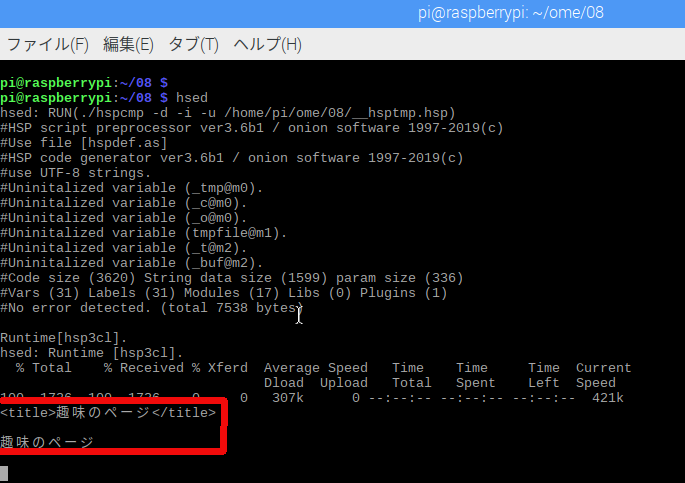
\includegraphics[width=15.411cm,height=11.841cm]{textbook-img015.png}

\end{center}

\bigskip


\bigskip


\bigskip

このようにさっきターミナルやテキストエディタで頑張って手動で行った動作をプログラムで行うことができました。
プログラムから情報を取り出すことができると、取り出した情報を使ってウェブページを作ったり、情報をもとにセンサーなどを操作できるようになります。
例えば、次の例で試すアメダスとよばれる気象情報観測システムの観測情報(気温、降水確率)などの情報を取り出し、LEDなどのセンサーと組み合わせます。
実現したいアイディアがあったらメモをしておきましょう。

\refstepcounter{Question}
\clearpage\subsection*{\theQuestion}
\begin{itemize}
\item
残りのグループ内の友達のウェブページのタイトルを取り出してみよう
\end{itemize}
\ \ HINT:
firend\_ipでダウンロードしたい友達のIPアドレスを指定する

\ \ \ \ メモした友達のIPアドレスを使おう

\refstepcounter{Question}
\subsection*{\theQuestion}
\begin{itemize}
\item 13行目 curl url, htmlの下の行にmes
htmlを追加して、実際にダウンロードされたHTMLを確認してみよう
\end{itemize}
\ \ HINT : 14行目にmes htmlを書く

\refstepcounter{Question}
\subsection*{\theQuestion}
\begin{itemize}
\item 15行目のhtmltag html, “title”,
tagの”title”を”ol”に変更してみましょう
\end{itemize}
\ \ HINT: htmltag html, “ol”, tag

\ \ htmltag html, “title”,
tag命令はtag変数の中に、
”{\textless}title{\textgreater}...{\textless}/title{\textgreater}”
を探した結果を入れています。
”title”を”ol”に変えると“
{\textless}ol{\textgreater}...{\textless}/ol{\textgreater}”
タグを探して、結果を入れてくれます。


\refstepcounter{Question}
\subsection*{\theQuestion}
\begin{itemize}
\item 15行目のhtmltag html, “title”,
tagの”title”を探したいタグへ変更しよう
\end{itemize}
\ \ HINT: pタグを探したい場合

\ \ \ \ \ htmltag html, “p”, tag


\bigskip

\clearpage\section{文字コードについて}
コンピュータは数字の0,
1しかわからないことを学びました。
0,1の2種類でなる数字列を2進数(バイナリ)といいます。
ところで、文字はどのように表示されているのでしょうか?そこで使われるのが文字コードです。
コンピュータは結局数値しかわからないので、数値と文字の対応を用いて、人間のわかる文字を表現します。
その対応にあたるものが文字コードで、数字列を文字に変換するルールです。

例えば、ASCIIでは英語のアルファベットをすべて表現できます。
ASCIIはアメリカで決められ、英語圏ではよく使われます。
ASCIIのテーブルをみて、表現を確認してみましょう。


\bigskip

{\bfseries
表のDecimalは10進数の数値,
Hex(Hexadecimal)は16進数の数値,
Char(Character)は文字を意味します。}


\bigskip

[\url{https://simple.wikipedia.org/wiki/ASCII}]

\begin{center}
  % Unhandled or unsupported graphics:
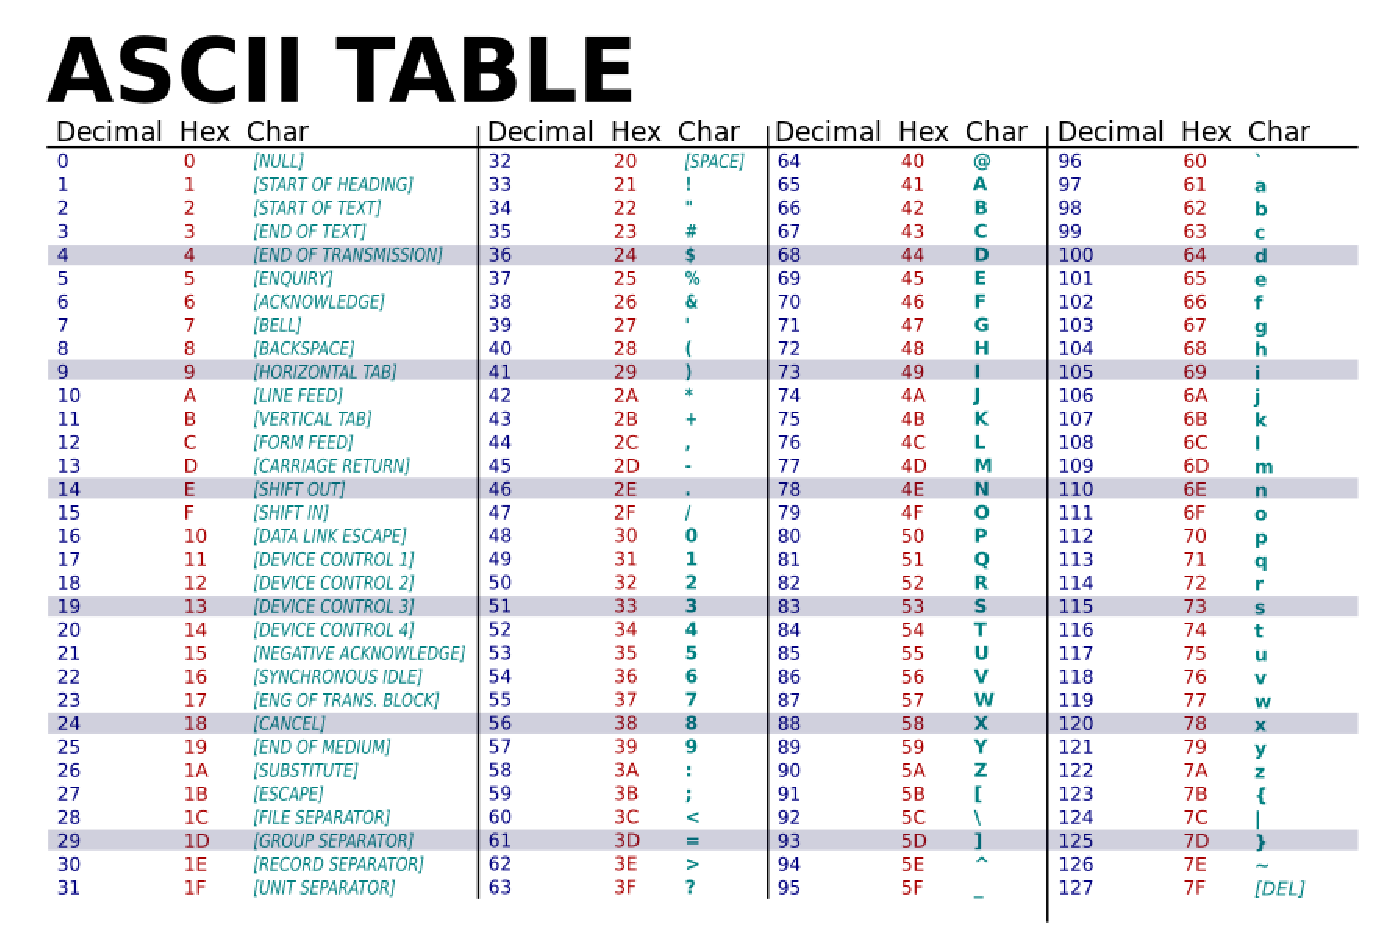
\includegraphics[width=17.006cm,height=11.317cm]{textbook-img016.eps}

\end{center}
ASCII
コードでは2進数7桁で一つの文字を表します。
128個の文字を表すことができます。


\bigskip


\bigskip


\bigskip

\clearpage
ASCIIでは0〜127を使用していました。
しかし、漢字などたくさんの文字がある日本語、中国語などではこの数値の範囲に収まりません。
いろいろな会社や組織が別々の方法で工夫して日本語を表現したので、異なる文字コードがあります。

代表的な文字コードと使いみちの例をあげます。

\begin{itemize}
\item Shift\_JIS 日本語版Windows・Mac
\item EUC-JP 旧UNIXワークステーション
\item ISO-2022-JP 電子メール
\item Unicode(UTF-8)
ラズベリーパイ、スマートフォン、海外版Windows


\bigskip
\end{itemize}

\bigskip
\refstepcounter{Exercise}
\clearpage\section{\theExercise 数字をASCIIを使って文字に変える}
考え方

\ \ printfコマンドを使用すると数字をASCIIに従って文字へ変換できます。
表のHEXの列をみて、41,
42,
43を探してみましょう。
何が表示されるか考えて試してみましょう。

ターミナルを開いて、

\ \ \textbf{printf “{\textbackslash}x41 {\textbackslash}x42 {\textbackslash}x43 {\textbackslash}n”}

を実行しましょう。

一番最後についている{\textbackslash}nは改行(カーソルを次の行に変える)という意味があります.

{\textbackslash}xはHE\textbf{X}(16進数であることを指定します)

\begin{center}
  % Unhandled or unsupported graphics:
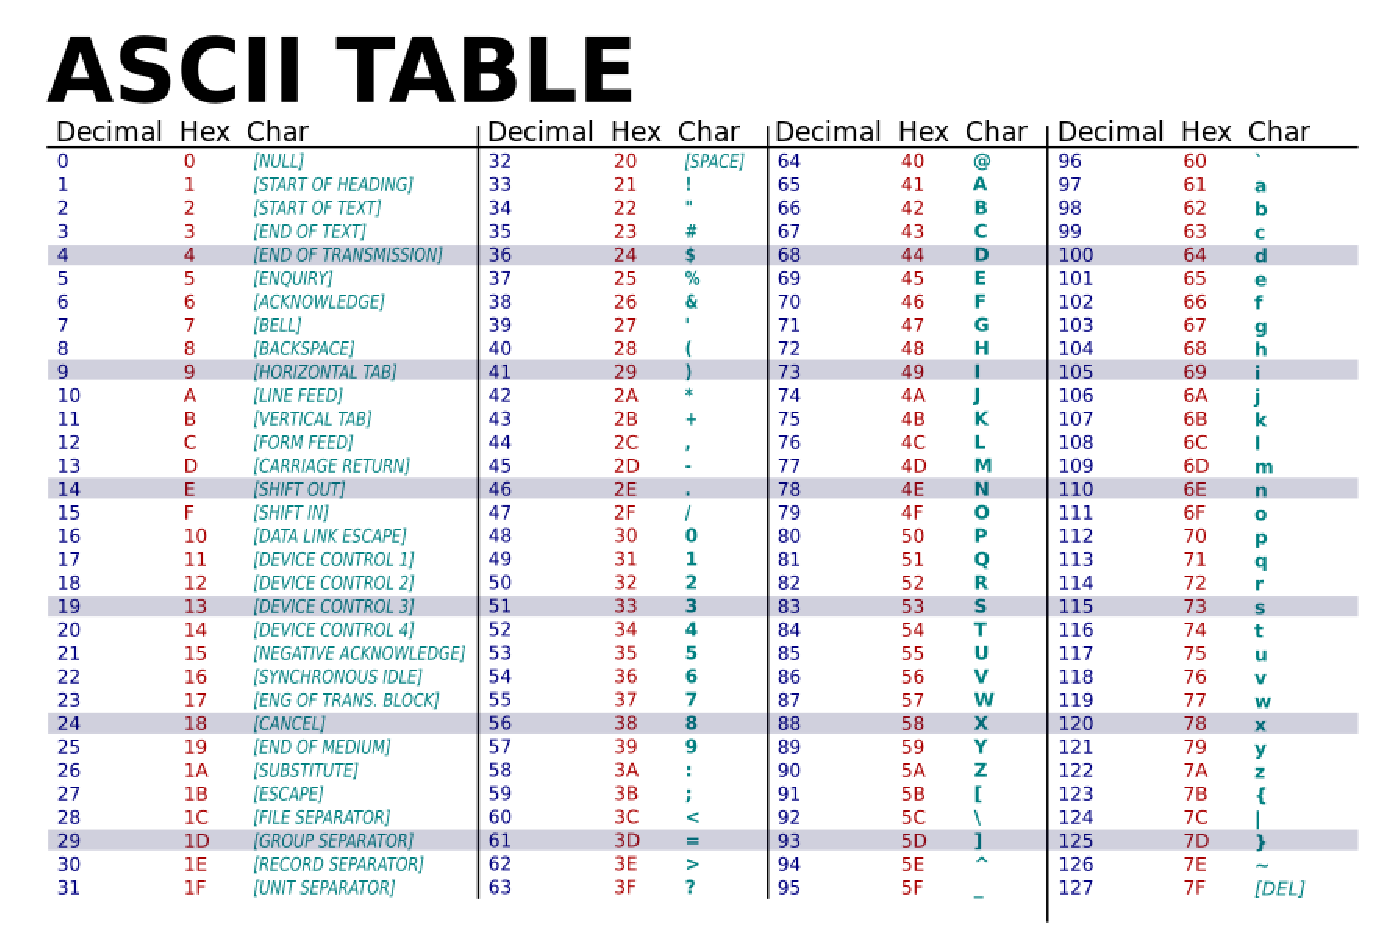
\includegraphics[width=17.006cm,height=11.317cm]{textbook-img016.eps}

\end{center}

\bigskip


\bigskip

{\bfseries
表のDecimalは10進数の数値,
Hex(Hexadecimal)は16進数の数値,
Char(Character)は文字を意味します。}

{\bfseries
[\url{https://simple.wikipedia.org/wiki/ASCII}]}

\refstepcounter{Question}
\clearpage\subsection*{\theQuestion}
\begin{itemize}
\item
ASCIIを使ってローマ字で自分の名前を表示させてみよう
\end{itemize}
\refstepcounter{Question}
\subsection*{\theQuestion}
\begin{itemize}
\item
ASCIIを使ってローマ字でとなりの友達の名前を表示させてみよう
\end{itemize}
\refstepcounter{Question}
\subsection*{\theQuestion}
\begin{itemize}
\item
ASCIIで顔文字を作って表示させてみよう
\end{itemize}
\ \ 例.) (* \^{} *) \ (* \_ *) \ (d\_b)


\bigskip

{\bfseries
表のDecimalは10進数の数値,
Hex(Hexadecimal)は16進数の数値,
Char(Character)は文字を意味します。}

\begin{center}
  % Unhandled or unsupported graphics:
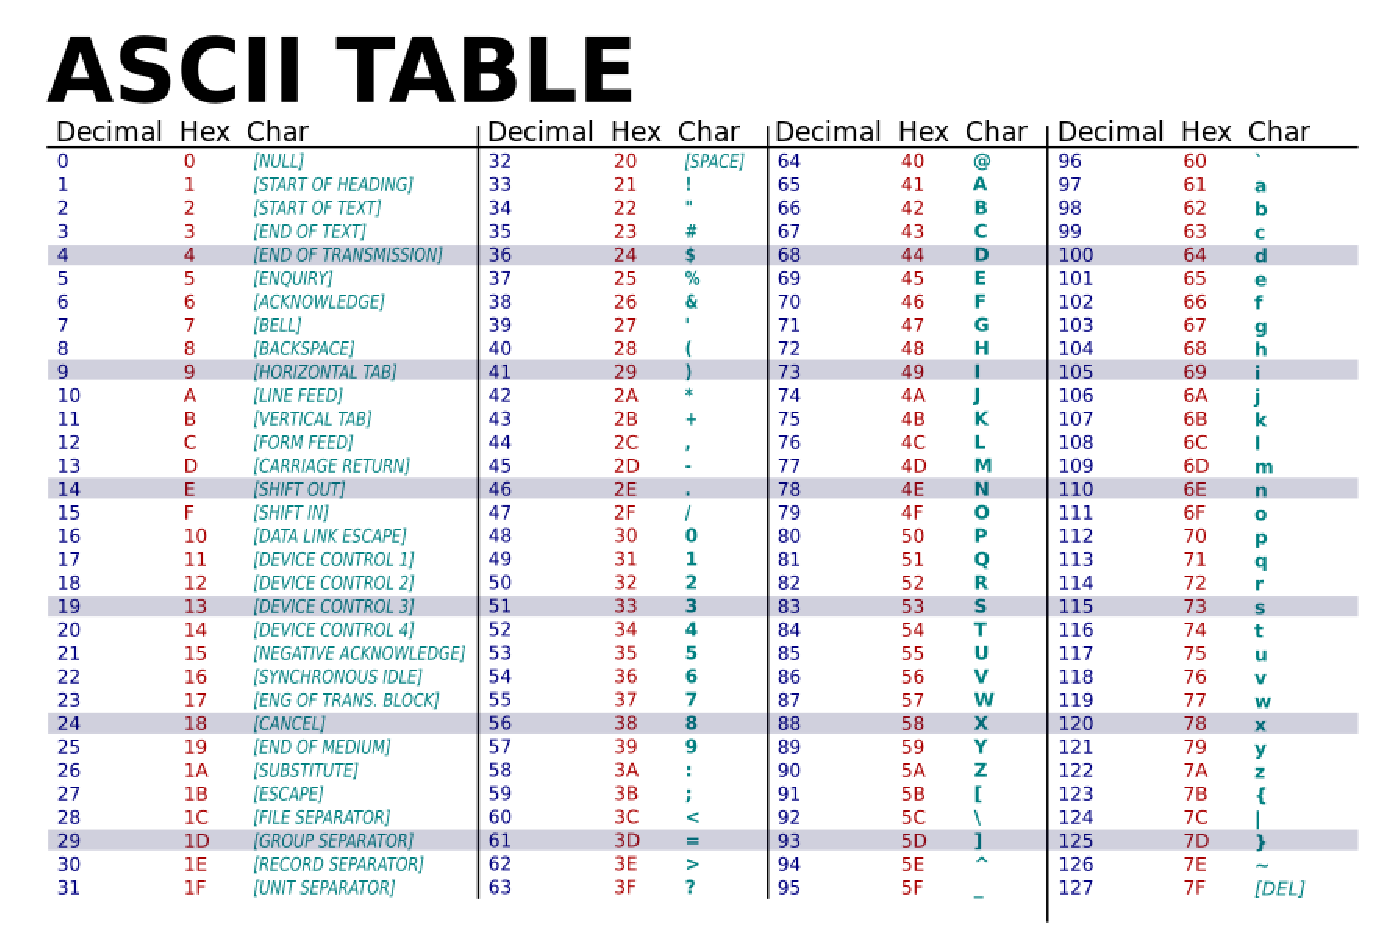
\includegraphics[width=17.006cm,height=11.317cm]{textbook-img016.eps}

\end{center}
{\bfseries
[\url{https://simple.wikipedia.org/wiki/ASCII}]}
\refstepcounter{Exercise}
\clearpage\section{\theExercise 数字をUTF-8を使って文字に変える}
\addtocounter{Exercise}{-1}\refstepcounter{Exercise}\label{E:UTF8}
考え方

\ \ printfコマンドを使用すると数字をUTF-8に従って文字に変換できます。
UTF-8は日本語も漢字を含め表現することができます。

授業で使用したホームページを開いてください。\textbf{(\~{}/08/links.html)}



\begin{center}
  % Unhandled or unsupported graphics:
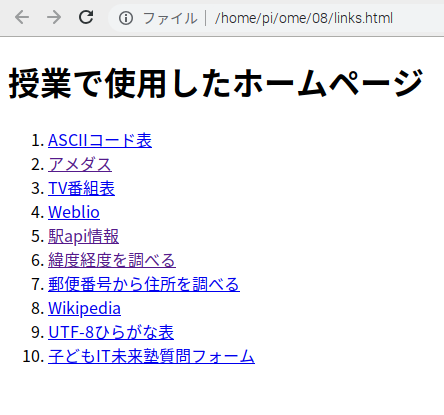
\includegraphics[width=9.398cm,height=8.784cm]{textbook-img017.png}

\end{center}


\bigskip


\bigskip

9.
UTF-8ひらがな表を開いてください。
UTF-8のひらがなに対応する数値の表があります。

”あ”を表示したい場合、”あ”がある行を見るとE3
81
80となっています。
列を見ると2となっています。
これらを足すと

E3 81 80 + 2 = E3 81 82

[\url{http://orange-factory.com/sample/utf8/code3/e3.html#Hiragana}]

\begin{center}
  % Unhandled or unsupported graphics:
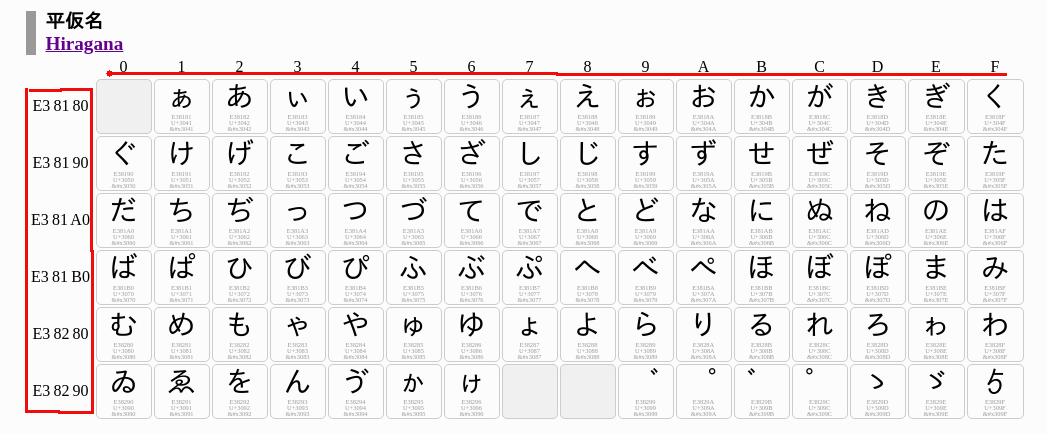
\includegraphics[width=17.006cm,height=7.049cm]{textbook-img018.png}

\end{center}
ターミナルを開いて、

\ \ \textbf{printf “{\textbackslash}xe3{\textbackslash}x81{\textbackslash}x82{\textbackslash}n”}

を実行しましょう。

一番最後についている{\textbackslash}nは改行(カーソルを次の行に変える)という意味があります.

{\textbackslash}xはHE\textbf{X}(16進数であることを指定します)

\refstepcounter{Question}
\clearpage\subsection*{\theQuestion}
\begin{itemize}
\item
UTF-8を使ってひらがなで自分の名前を表示させてみよう
\end{itemize}
\refstepcounter{Question}
\subsection*{\theQuestion}
\begin{itemize}
\item
UTF-8を使ってひらがなでとなりの友達の名前を表示させてみよう
\end{itemize}

\bigskip



\begin{center}
  % Unhandled or unsupported graphics:
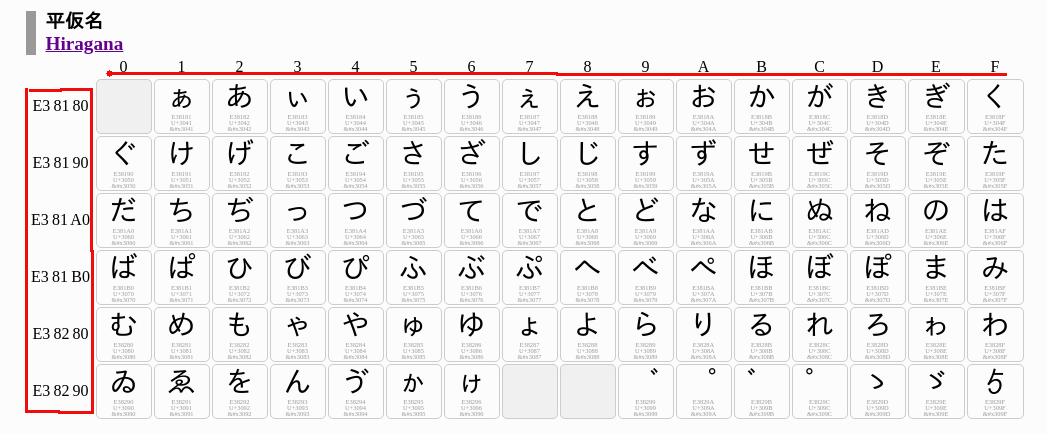
\includegraphics[width=17.006cm,height=7.049cm]{textbook-img018.png}

\end{center}

\bigskip

[\url{http://orange-factory.com/sample/utf8/code3/e3.html#Hiragana}]
\refstepcounter{Exercise}
\clearpage\section{\theExercise ウェブページで使用されている文字コードを変換する}
考え方

ある文字コードで表現された文字列を他の文字コードで解釈すると文字化けをする可能性があります。
例えば、UTF-8と設定されたターミナルなどのアプリケーションでEUC-JPで書かれたファイルを開くなどすると文字化けをします。
これは、文字を表現するのに2つの文字コード間で数値が違うからです。
ターミナルなどのアプリケーションから正しく扱うためには、ターミナルやアプリケーションが使っている文字コードに変換する必要があります。
この例では変換の練習をします。

ターミナルが使っている文字コードを確認してみよう

echo \$LANG

jp\_ja.UTF-8

\begin{center}
  % Unhandled or unsupported graphics:
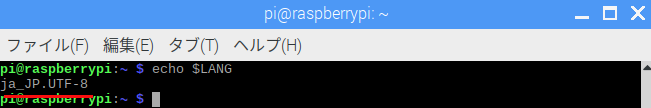
\includegraphics[width=17.006cm,height=3.231cm]{textbook-img019.png}

\end{center}
国\_言語.文字コード

のように表されています。
ターミナルはUTF-8の文字コードを使用しています。
LANGは(環境)変数で、アプリケーションやコマンドが使用するロケール(国や地域によって異なる言語や単位、日付などの表記など)の設定をします。


LANGに設定されている文字コードと表示したい文字コードが異なっていると、文字化けをします。例えば、UTF-8を使っているシステムで、EUC-JPで表現された文字列を表示した場合など。


試しにUTF-8以外の文字コードを使用しているウェブサイトをcurlでダウンロードして、UTF-8として設定されているターミナルに表示させてみよう

\textbf{cd \~{}/08}

curl \url{http://x68000.q-e-d.net/~68user/unix/pickup?iconv} -o hsp.html

\begin{center}
  % Unhandled or unsupported graphics:
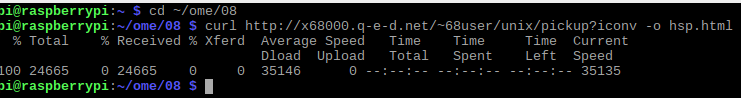
\includegraphics[width=17.006cm,height=3.53cm]{textbook-img020.png}

\end{center}

\bigskip

\clearpage
lessで開いてみよう

less hsp.html



\begin{center}
  % Unhandled or unsupported graphics:
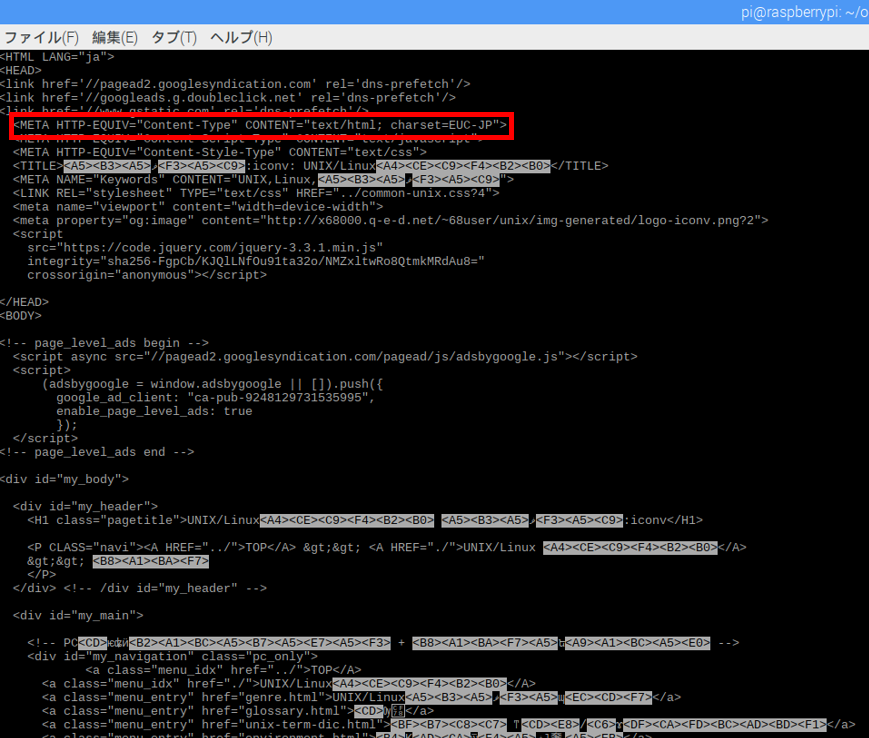
\includegraphics[width=17.006cm,height=12.086cm]{textbook-img021-1.png}

\end{center}
{\textless}meta
charset=”EUC-JP”{\textgreater}という行を探してみよう。

{\textless}head{\textgreater}{\textless}/head{\textgreater}タグの中に入っているので、先頭のほうにあります。

このHTMLファイルはEUC-JPという文字コードが使われています。

ファイルの中を見てみると、文字化けしている箇所があります。



\begin{center}
  % Unhandled or unsupported graphics:
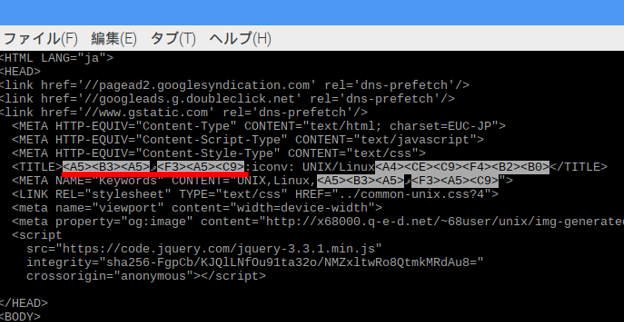
\includegraphics[width=17.006cm,height=5.63cm]{textbook-img021-2.png}

\end{center}
UTF-8を使っているターミナルへEUC-JPで記述されたファイルの中身を表示したので、このように文字化けしてしまいます


\bigskip


\bigskip

\clearpage
文字化けを解消するために、EUC-JPからUTF-8へ変換してみよう

\textbf{iconv hsp.html -f EUC-JP -t UTF-8 -o hsp\_utf8.html}

\begin{center}
\begin{boxedminipage}{17.228cm}
\section*{コラム
iconvコマンドのオプション(機能)}
iconvのオプションについて

{}-fオプションでは変換前の文字コードを指定します。

{}-tオプションでは変換後の文字コードを指定します

{}-oオプションはcurlと同じで、出力ファイル名を指定します。

iconv hsp.html -f EUC-JP -t UTF-8 -o hsp\_utf8.html

では、hsp.htmlをEUC-JPからUTF-8に変換してhsp\_utf8.htmlとして出力するという意味になります。
\end{boxedminipage}
\end{center}
\begin{center}
  % Unhandled or unsupported graphics:
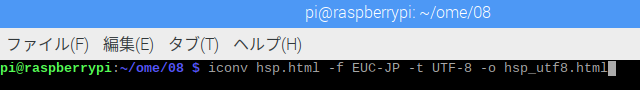
\includegraphics[width=17.006cm,height=2.164cm]{textbook-img022.png}

\end{center}
変換ができたら、同様にlessコマンドで見てみよう

\textbf{less hsp\_utf8.html}



\begin{center}
  % Unhandled or unsupported graphics:
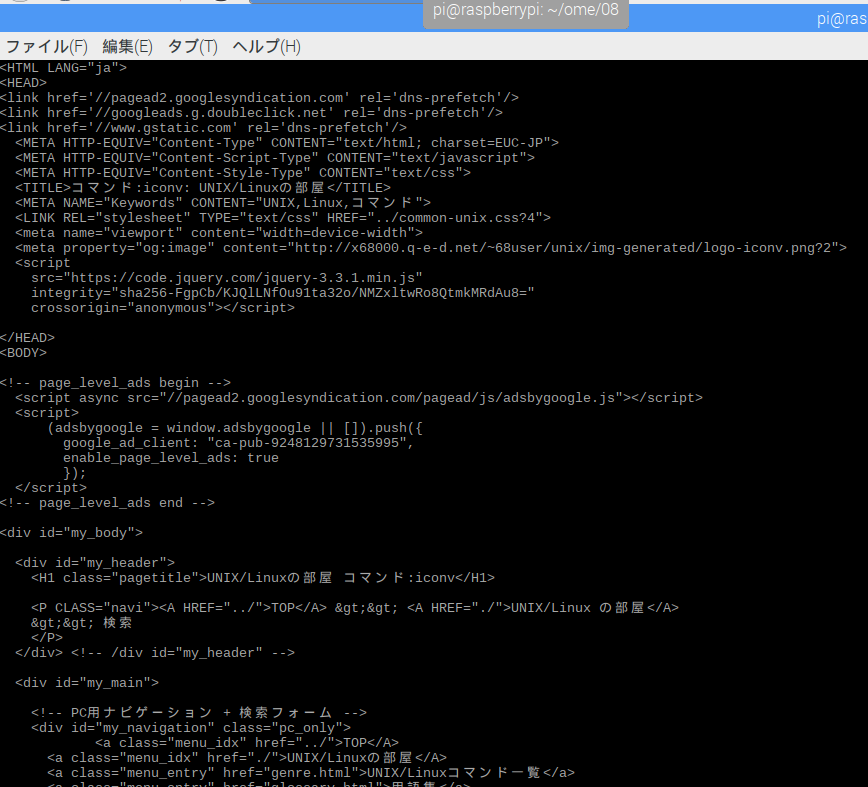
\includegraphics[width=17.006cm,height=12.086cm]{textbook-img023.png}

\end{center}
変換したファイルでは文字化けはしていません。
文字コードの変換ができました。

\clearpage
しかし、HTMLファイルは{\textless}meta
charset=””{\textgreater}で文字コードを指定しています。
ブラウザやHTMLを扱うソフトウェアの多くはここに書かれている文字コードを使用してHTMLを理解します。

試しに、UTF-8に変換したHTMLファイル\textbf{(\~{}/08/hsp\_utf8.html)}をブラウザで開いてみよう。

ブラウザを開いて、

\textbf{\~{}/08/hsp\_utf8.html} と入力しエンターを押します。

\begin{center}
  % Unhandled or unsupported graphics:
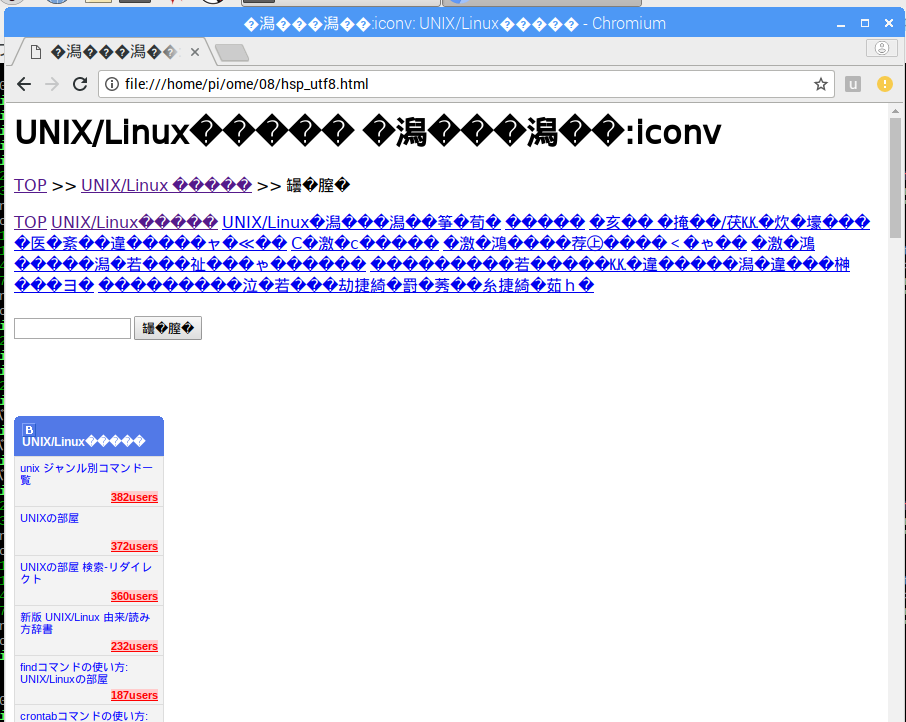
\includegraphics[width=16.113cm,height=11.518cm]{textbook-img024.png}

\end{center}
表示されているほとんどが、文字化けしています。
画像はダウンロードしていないので表示されません。
これは、ファイルの中身をUTF-8に変換したけれど、ブラウザやHTMLを扱う多くのソフトウェアは{\textless}meta
charset=””{\textgreater}を確認して文字コードを判断します。
ここを修正しなければ、正しく扱われません。
このタグで指定している文字コードを変換後の文字コードであるUTF-8に変更して置く必要があります。


ターミナルで、

leafpad



\begin{center}
  % Unhandled or unsupported graphics:
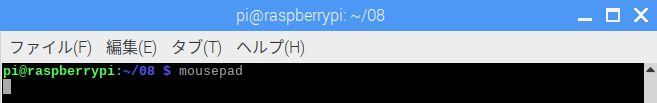
\includegraphics[width=17.006cm,height=2.87cm]{textbook-img006.png}

\end{center}
\clearpage
ファイル→ 開くから

hsp\_utf8.htmlを開きます。

charset=”EUC-JP”を探して、



\begin{center}
  % Unhandled or unsupported graphics:
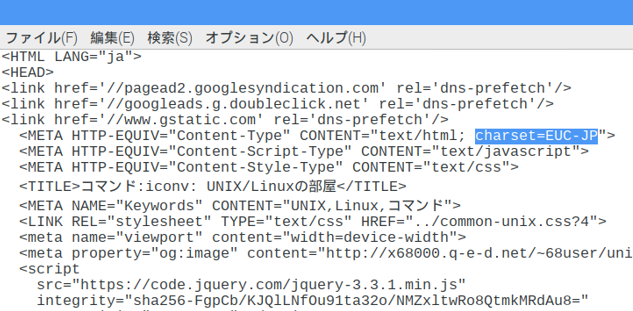
\includegraphics[width=17.006cm,height=4.417cm]{textbook-img025.png}

\end{center}
charset=”UTF-8”に変更します。



\begin{center}
  % Unhandled or unsupported graphics:
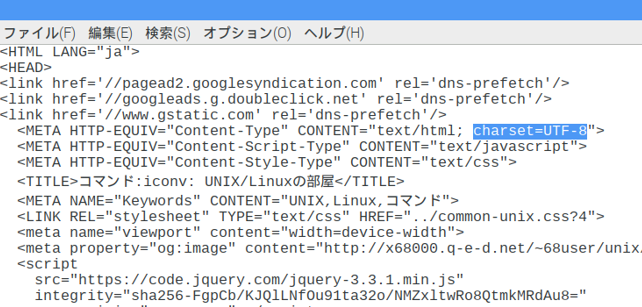
\includegraphics[width=17.006cm,height=4.567cm]{textbook-img026.png}

\end{center}
保存してブラウザをリロードすると



\begin{center}
  % Unhandled or unsupported graphics:
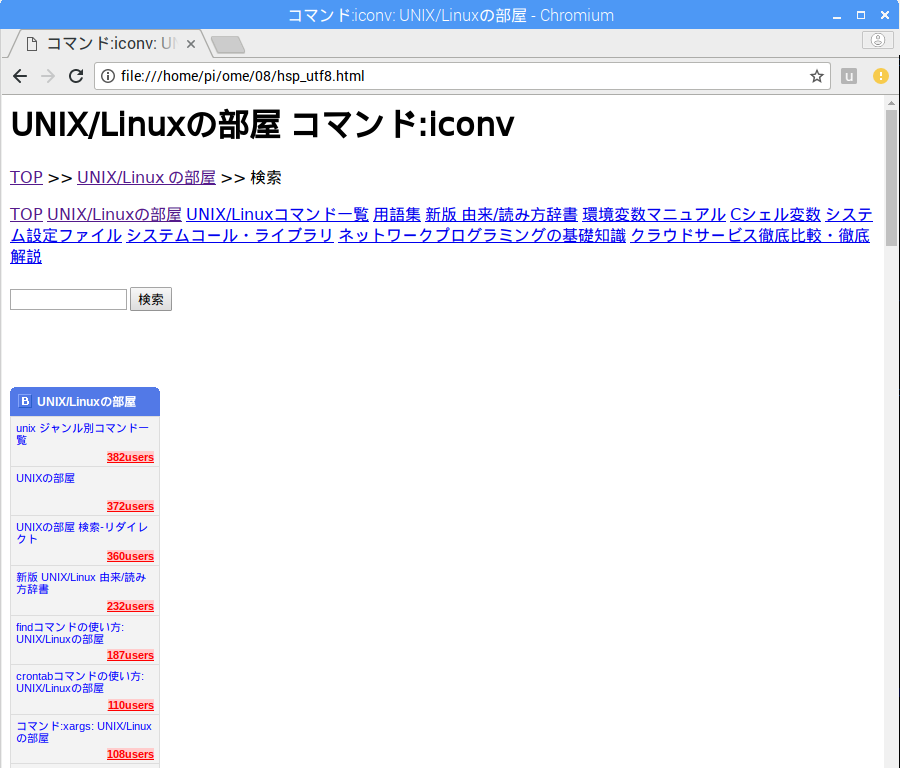
\includegraphics[width=12.495cm,height=7.932cm]{textbook-img027.png}

\end{center}


\bigskip


\bigskip

文字化けせずに正しく表示されました。
HTMLファイルの文字コードを変換するときは、{\textless}meta
charset=””{\textgreater}を変換後の文字コードに変更するのを忘れないようにしましょう。

\clearpage\section{スクレイピング}
クレイピングとは、ウェブページから情報を取り出すことをいいます。
スクレイピングの手順はウェブページをダウンロードして、ウェブページから欲しい情報を探して取り出し、そして、取り出し情報を加工します。
\ref*{E:CURL},\ref*{E:HTML}
で手動でウェブページをダウンロードして、そこから情報を取り出しました。
そのあとの\ref*{E:SCRAPING}では、同じ手順をプログラムで自動で行いました。
ウェブページから取り出した情報をプログラムから有効的に使う方法を学びましょう。
ウェブページから取り出した情報をもとにセンサーを使ったり、情報をウェブページに反映することもできます。
ウェブページから価値のある情報を取り出して、今まで習った技術と組み合わせて役に立つプログラムを作れるように考えながら例題を進めていきましょう。



\bigskip
\refstepcounter{Exercise}
\clearpage\section{\theExercise アメダスのウェブページをスクレイピングする}
%\newline
考え方

まずは、ウェブブラウザでアメダスのページを見てみよう。
授業で使用したホームページを開いてください。
\textbf{(\~{}/08/links.html)}

アメダスをクリックします。 



\begin{center}
  % Unhandled or unsupported graphics:
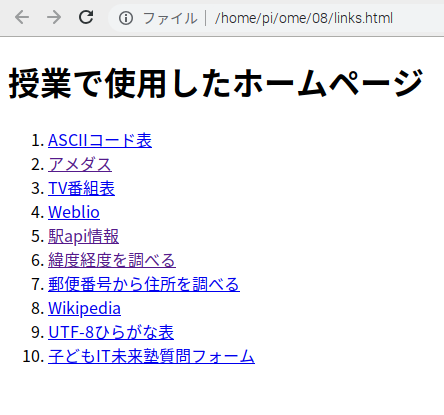
\includegraphics[width=9.398cm,height=8.784cm]{textbook-img017.png}

\end{center}


\bigskip


\bigskip

アメダスのウェブページが開きます。

\begin{center}
  % Unhandled or unsupported graphics:
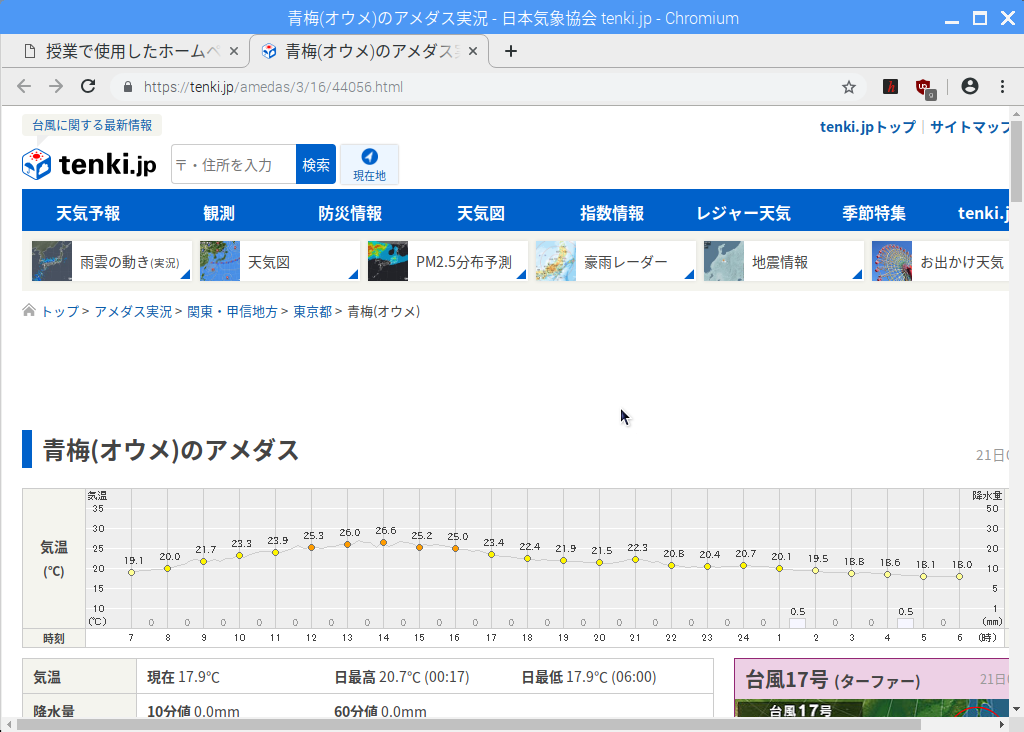
\includegraphics[width=17.006cm,height=12.157cm]{textbook-img028.png}

\end{center}
\clearpage
少ししたのほうに”アメダス履歴(10分観測値)”という見出しがあります。

青梅市のアメダス観測データを10分毎に表にしたものです。



\begin{center}
  % Unhandled or unsupported graphics:

\includegraphics[width=17.006cm,height=12.157cm]{textbook-img029.png}

\end{center}
今回はこの表から最新の10分観測値の情報を自動でプログラムから取得して、さらに取得した情報をプログラムで利用します。



\begin{center}
  % Unhandled or unsupported graphics:
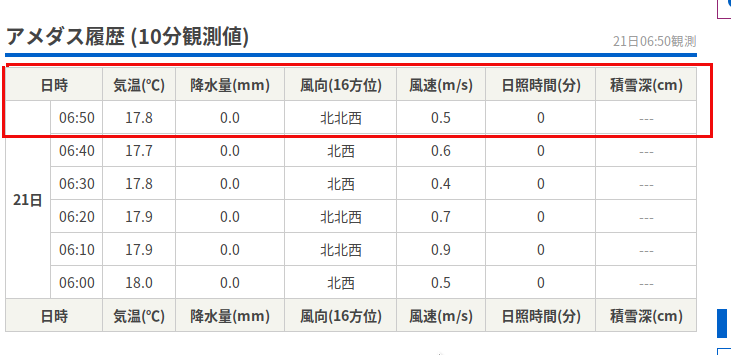
\includegraphics[width=17.006cm,height=5.777cm]{textbook-img029-1.png}

\end{center}

\bigskip

\clearpage
まずはプログラムを動かしてみましょう。

ターミナルを開いて

hsed

と実行します



\begin{center}
  % Unhandled or unsupported graphics:
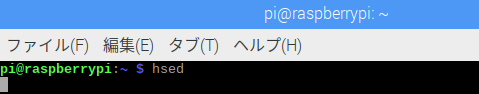
\includegraphics[width=13.28cm,height=2.933cm]{textbook-img013.png}

\end{center}

\bigskip


\bigskip


\bigskip

HSPスクリプトエディタが開くので

ファイル → 開く.. 

をクリックして\textbf{\~{}/08/amedas.hsp}を開きます。

プログラムが表示されます。



\begin{center}
  % Unhandled or unsupported graphics:
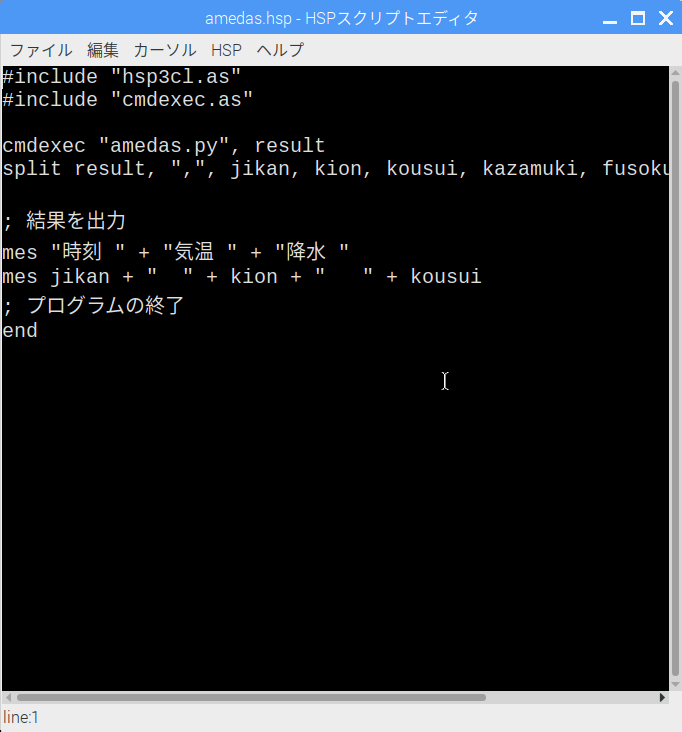
\includegraphics[width=13.887cm,height=14.903cm]{textbook-img030.png}

\end{center}

\bigskip


\bigskip

\clearpage
F5を押して実行してみましょう。実行結果はターミナルに表示されます。



\begin{center}
  % Unhandled or unsupported graphics:
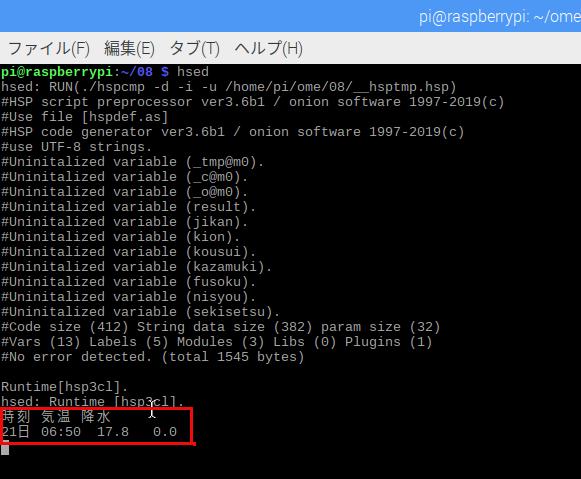
\includegraphics[width=16.722cm,height=11.229cm]{textbook-img031.png}

\end{center}

\bigskip


\bigskip

表示されている時刻、気温、降水とブラウザで見たアメダスの情報を比べてみてください。



\begin{center}
  % Unhandled or unsupported graphics:
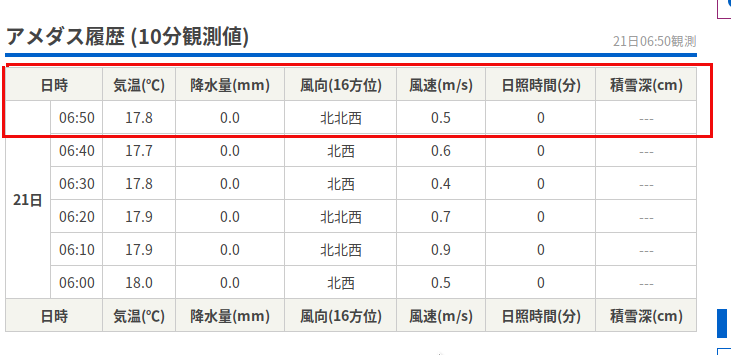
\includegraphics[width=17.006cm,height=5.777cm]{textbook-img029-1.png}

\end{center}
同じ値が表示されています。
このようにHSPのプログラムでウェブページからアメダスの情報を取得することができました。


\bigskip

\clearpage
プログラム解説

この例題プログラムでは、amedas.pyというコマンドを使って、ウェブページからアメダスの情報を取得しています。

\begin{center}
\begin{boxedminipage}{17.126cm}
\begin{enumerate}
\baselineskip 10pt
\setlength{\itemsep}{0cm} % 項目間
\item \#include {\textquotedbl}hsp3cl.as{\textquotedbl}
\item \#include {\textquotedbl}cmdexec.as{\textquotedbl}
\item 
\item cmdexec {\textquotedbl}amedas.py{\textquotedbl}, result
\item split result, {\textquotedbl},{\textquotedbl}, jikan, kion, kousui, kazamuki, fusoku, nisyou, sekisetsu
\item 
\item ; 結果を出力
\item mes {\textquotedbl}時刻 {\textquotedbl} + {\textquotedbl}気温 {\textquotedbl} +
{\textquotedbl}降水 {\textquotedbl} \ 
\item mes jikan + {\textquotedbl} \ {\textquotedbl} + kion + {\textquotedbl} \ \ {\textquotedbl} + kousui
\item ; プログラムの終了
\item end
\end{enumerate}
\end{boxedminipage}
\end{center}
4行目でHSPプログラム内からamedas.pyコマンドを実行しています。

cmdexec命令は、execと基本的には同じですが、実行するコマンドの後に変数名をつけます。
この変数にはコマンドの実行結果が文字列で入ります。

一度、amedas.pyコマンドをターミナルで実行してみましょう。
ターミナルを開きます。

amedas.py を実行します。

カンマ(,)で区切られて値が表示されています。

\begin{center}
  % Unhandled or unsupported graphics:
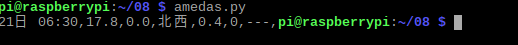
\includegraphics[width=17.006cm,height=1.122cm]{textbook-img032-1.png}

\end{center}
これらの値がなにを意味しているのか見てみましょう。

\textbf{amedas.py \ {}-{}-print-headers}

を実行します。



\begin{center}
  % Unhandled or unsupported graphics:
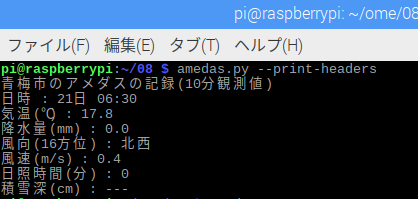
\includegraphics[width=17.006cm,height=5.237cm]{textbook-img032-2.png}

\end{center}
日時、気温、降水量、風向、風速、日照時間、積雪深の順番で値と値の見出しが表示されています。

このカンマ(,)区切りの数値も同じ並びで表示されています。

HSPのプログラムに戻ります。

\begin{center}
  % Unhandled or unsupported graphics:
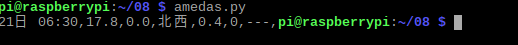
\includegraphics[width=17.006cm,height=1.122cm]{textbook-img032-1.png}

\end{center}
5行目で、カンマ(,)で区切られた実行結果を分解してそれぞれ変数へいれています。

結果は日時、気温、降水量、風向き、風速、日照、積雪深の順になっているので、

split result, {\textquotedbl},{\textquotedbl}, jikan, kion, kousui, kazamuki, fusoku, nisyou, sekisetsu


\bigskip

\begin{center}
\tablefirsthead{}
\tablehead{}
\tabletail{}
\tablelasttail{}
\begin{supertabular}{|m{16.806cm}|}
\hline
split命令の使い方

split 分解前の変数(文字列), \ “区切り文字”,
変数..

例 : 

split “りんご,ぶどう,オレンジ”, \ “,”, apple, grape, orange

\ 文字列を
カンマ(,)で区切って順番に変数にいれている

apple ← “りんご”

grape ← “ぶどう”

orange ← “オレンジ”\\\hline
\end{supertabular}
\end{center}

\bigskip


\bigskip

変数の順番も対応させます。

日時  → \ jikan

気温  → kion  

降水 → kousui 

風向き→ kazamuki

風速 → fusoku

日照 → nisyou

積雪深→ sekisetsu

変数に文字列として入れています。


\bigskip

9行目で日時(jikan), 気温(kion),
降水(kousui)を表示させています。

mes jikan + {\textquotedbl} \ {\textquotedbl} + kion + {\textquotedbl} \ \ {\textquotedbl} + kousui

\refstepcounter{Question}
\clearpage\subsection*{\theQuestion}
\begin{itemize}
\item
.例題のプログラムでは、日時、気温、降水だけ表示しています。
		プログラムでは、風向き、風速、日照も取得してます。
		これらも表示させてみましょう。
\end{itemize}
\ \ HINT : それぞれkazamuki, fusoku,
nisyouという変数に情報が入っています。

\refstepcounter{Question}
\subsection*{\theQuestion}
\begin{itemize}
\item
kionが25.0度以上のときに、現在の気温を表示し、センサーボードの赤色LEDをつけてみましょう。
		それ以外の場合は、画面に現在の気温を表示し、白色LEDをつけましょう。
\end{itemize}
\ \ HINT :
例題プログラムのkionを数値へ変換してみましょう。

\ \ HINT :
プログラムに応用するには大小の比較とかできると便利です。
大小比較をするには文字列から数値へ変換が必要です

\ \ HSPでは、文字列で表された数値はdouble関数を使って文字列から数値へ変換できます。

\ \ 例えば、



\begin{center}
\begin{boxedminipage}{8.326cm}
\begin{enumerate}
\baselineskip 10pt
\setlength{\itemsep}{0cm} % 項目間
\item kion = “28.2”
\item kion = double(kion)
\end{enumerate}
\end{boxedminipage}
\end{center}

\bigskip


\bigskip

\refstepcounter{Question}
\subsection*{\theQuestion}
\begin{itemize}
\item
このアメダスのスクレイピングの例題とすでに習った技術(センサーボードの使い方、ゲーム、Fabo、赤外線など)と組み合わせるとどんなことができるか考えて、1つ上げてみよう。
\end{itemize}

\bigskip


\bigskip

\clearpage\section{スクレイピングの仕組み}
\ref*{E:SCRAPING}でHSPのプログラムから友達のウェブページのタイトルを取り出したように、スクレイピングでは、HTMLファイルのタグ(\ref*{E:SCRAPING}では{\textless}title{\textgreater}{\textless}/title{\textgreater})を探します。
しかし、ウェブページの欲しい情報はHTMLファイル内のどのタグで作られているでしょうか?ウェブページをダウンロードして、HTMLファイルを眺めても探しても良いのですが、かなり大変です。
ここでは、ウェブページの欲しい情報がどのHTMLファイル内のどのタグで作られているか調べる方法としてブラウザの検証ツールを使った方法を紹介します。
アメダスのウェブページを例に試していきます。


\bigskip

まずは、ウェブブラウザでアメダスのページを見てみよう。
授業で使用したホームページを開いてください。
\textbf{(\~{}/08/links.html)}

アメダスをクリックします。 



\begin{center}
  % Unhandled or unsupported graphics:
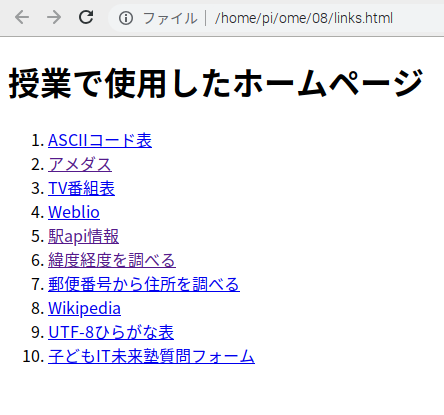
\includegraphics[width=6.271cm,height=5.86cm]{textbook-img017.png}

\end{center}

\bigskip


\bigskip



アメダスのウェブページが開きます。

\begin{center}
  % Unhandled or unsupported graphics:
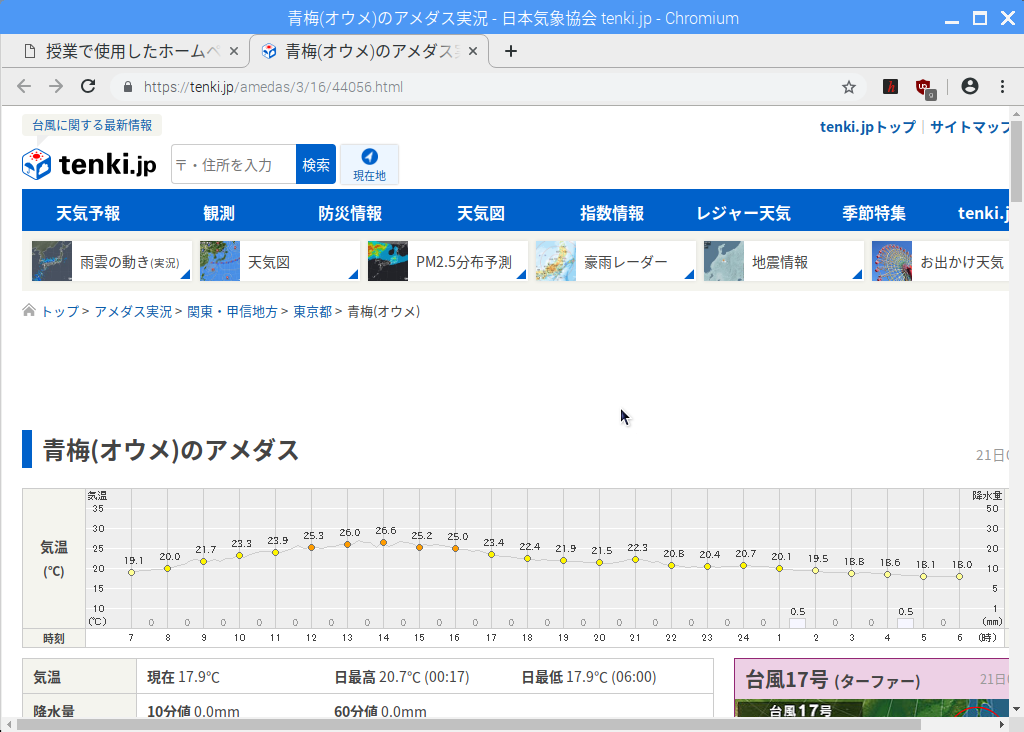
\includegraphics[width=14.252cm,height=9.687cm]{textbook-img028.png}

\end{center}

\bigskip

\clearpage
少ししたのほうに”アメダス履歴(10分観測値)”という見出しがあります。

青梅市のアメダス観測データを10分毎に表にしたものです。



\begin{center}
  % Unhandled or unsupported graphics:
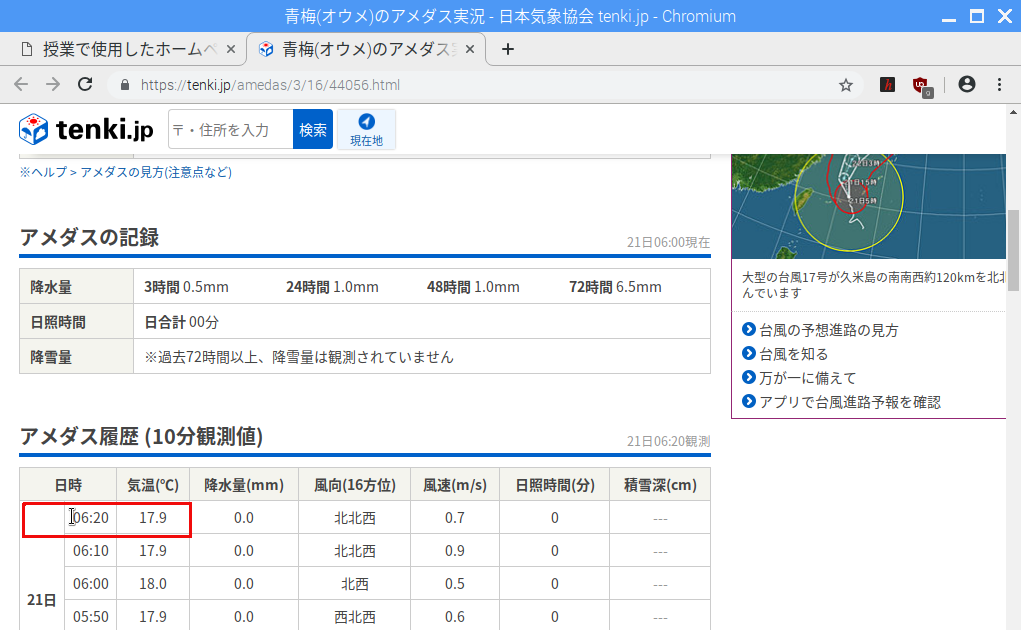
\includegraphics[width=17.006cm,height=10.433cm]{textbook-img033.png}

\end{center}
10分観測値の表の一番上の行にある、時刻にカーソルを合わせます。
ウェブページを開いた時間によって、表示が変わりますので、値が違っても気にしないでください。

カーソルを合わせたら、左クリックして、メニューを開き、”検証”をクリックします。

\begin{center}
  % Unhandled or unsupported graphics:
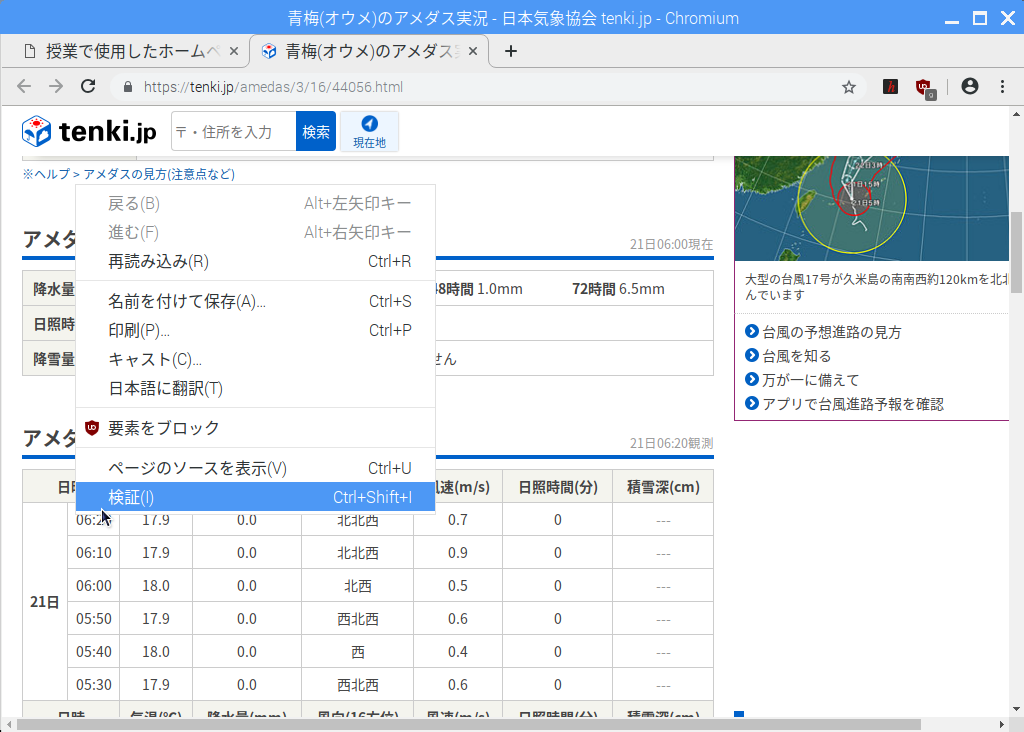
\includegraphics[width=17.006cm,height=9.843cm]{textbook-img034.png}

\end{center}
\clearpage
検証をクリックすると検証ツールが開きます。



\begin{center}
  % Unhandled or unsupported graphics:
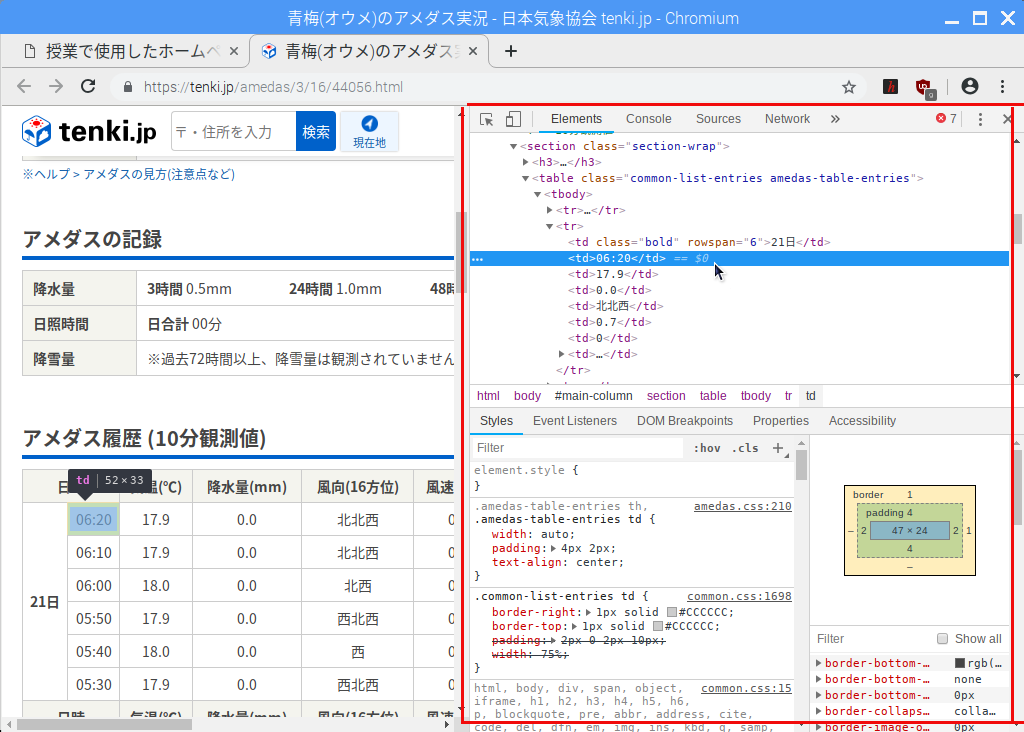
\includegraphics[width=17.006cm,height=12.157cm]{textbook-img035.png}

\end{center}
検証ツールにはウェブページのHTMLが上半分に表示されています。
現在、カーソルが乗っている(青くなっている)行に対応するウェブページが青く色づけされています。



\begin{center}
  % Unhandled or unsupported graphics:
\includegraphics[width=17.006cm,height=9.643cm]{textbook-img035-2.png}

\end{center}
現在、選択しているのは{\textless}td{\textgreater}{\textless}/td{\textgreater}タグです。
{\textless}td{\textgreater}{\textless}/td{\textgreater}タグ(table
data,
表の値)は表の値にあたる部分を書くときに使用します。

{\textless}tr{\textgreater}{\textless}/tr{\textgreater}タグ(table row,
表の行)は表の1行分を書くときに使います。
{\textless}tr{\textgreater}{\textless}/tr{\textgreater}タグの中に{\textless}td{\textgreater}{\textless}/td{\textgreater}タグを入れて、1行分の表の値を表します。


表は{\textless}table{\textgreater}{\textless}/table{\textgreater}タグ(table,
表)で作りました。


アメダスのサイトから情報を取り出す際には、まずは、{\textless}table{\textgreater}{\textless}/table{\textgreater}タグを探して取り出します。
{\textless}table{\textgreater}{\textless}/table{\textgreater}タグを取り出したあと、その中から、{\textless}tr{\textgreater}{\textless}/tr{\textgreater}タグを取り出して、さらに{\textless}td{\textgreater}{\textless}/td{\textgreater}タグを取り出し、実際の値を取り出すということを行っています。


実際に実行しているamedas.pyコマンドはだいたいこのような流れでアメダスのサイトの表から気温などの情報を取り出しています。


\bigskip


\bigskip



\begin{center}
  % Unhandled or unsupported graphics:
\includegraphics[width=16.178cm,height=12.051cm]{textbook-img035-3.png}

\end{center}
ちなみに、{\textless}table class=”common-list-entries amedas-table-entries”{\textgreater}

のようにタグに情報がついています。
classはいわば名前のようなもので、このタグについている情報を使ってタグをHTMLファイルから取り出すのが良いです。
このウェブページには、表が何個もあるので、{\textless}table{\textgreater}{\textless}/table{\textgreater}タグだけでは、すべての表が当てはまります。
しかし、このように名前などタグについた情報を一緒に指定することで、取りたいタグをより限定的にできます。


\bigskip


\bigskip
\refstepcounter{Exercise}
\clearpage\section{\theExercise amedas.pyをlessで見てみよう}
「スクレイピングの仕組み」では、アメダスのウェブページからアメダス観測値を取得する流れを解説しました。
実際にウェブページから値を取り出すのに使用しているコマンド(プログラム)を見てみましょう。
amedas.pyコマンドはHSPのプログラムから呼び出しているものです。

このプログラムはPython
2(パイソン)という言語で書かれています。
HSPとは書き方が違うので少し難しいかもしれないですが、プログラムの内容が理解できなくても、問題はないので気楽に見てみましょう。


\bigskip

amedas.pyコマンドもHSPのプログラムと同じくテキストファイルとして記述されています。

まずは、amedas.pyコマンドをlessコマンドで開きます。


\bigskip

\textbf{less \~{}/bin/amedas.py}



\begin{center}
  % Unhandled or unsupported graphics:
\includegraphics[width=17.006cm,height=2.067cm]{textbook-img036.png}

\end{center}
\begin{center}
  % Unhandled or unsupported graphics:
\includegraphics[width=17.006cm,height=9.086cm]{textbook-img037.png}

\end{center}
{\bfseries
(lessコマンドの詳しい使い方は3回目の教科書「2.2.12
ファイルの中身を見てみよう(2)」を見てください)%
%来年度、2.2.12を統一された例題番号へ変更する
%koyaman 
%September 23, 2019 8:47 PM
}


\bigskip

\clearpage
実際のスクレイピングの処理は30行目から下です。

35行目でhtmlを取得しています。

\begin{center}
\begin{boxedminipage}{16.947cm}
\begin{enumerate}
\setlength{\itemsep}{0cm} % 項目間
\setcounter{enumi}{29}
\item def main():
\item \ \ \ \ \#アメダスのウェブページのURL
\item \ \ \ \ url = 'http://tenki.jp/amedas/3/16/44056.html'
\item 
\item \ \ \ \ parse\_opts()
\item \ \ \ \ html = urllib2.urlopen(url).read()
\item \ \ \ \ soup = BeautifulSoup(html, 'html.parser')

\ \ \ \ …
\end{enumerate}
\end{boxedminipage}
\end{center}
HTMLからタグを探したりするソフトウェア(ライブラリ)にはBeautiful
Soupを使用しています。

38行目では、最初の{\textless}table class={\textquotedbl}common-list-entries
amedas-table-entries{\textquotedbl}{\textgreater}を探して取り出しています。

40行目では、取り出した{\textless}table{\textgreater}タグから{\textless}tr{\textgreater}タグを2行分取り出しています。

45行目で、値の説明(日時、気温、降水などの文字列)

\begin{center}
\begin{boxedminipage}{17.658cm}
\begin{enumerate}
\setlength{\itemsep}{0cm} % 項目間
\baselineskip 10pt
\setcounter{enumi}{36}
\item \# 最初の{\textless}table class={\textquotedbl}common-list-entries
amedas-table-entries{\textquotedbl}{\textgreater} ... {\textless}/table{\textgreater}を探す
\item \ \ \ \ table = soup.find\_all('table', attrs=\{'class' : 'common-list-entries amedas-table-entries'\})[0] 
\item \ \ \ \ \# 2行分取り出す
\item \ \ \ \ tr = [i for i in table.find\_all('tr')[:2]] \#
ヘッダー、値の2行
\item \ \ \ \ result = []
\item \ \ \ \ for i in tr:
\item \ \ \ \ \ \ \ \ result.append(i.text.strip())
\item \ \ \ \ \# 結果をヘッダーと値に分ける
\item \ \ \ \ headers = [i for i in result[0].splitlines()]
\item \ \ \ \ data \ \ \ = [i for i in result[1].splitlines()]
\end{enumerate}
\end{boxedminipage}
\end{center}
46行目で、値(21日6:20、17.9、0.0など値)

それぞれ{\textless}tr{\textgreater}タグから{\textless}td{\textgreater}の値を取り出しています。


あとは、カンマ(,)区切りで表示しているだけです。
「スクレイピングの仕組み」で説明した流れで実際にプログラムが書かれています。



\bigskip


\bigskip

サンプルプログラム、Pythonのことをもっと詳しく知りたい人はブラウザで

\begin{itemize}
\item Python 2
\item Python 2 スクレイピング
\item Python 2 Beautiful Soup4
\end{itemize}
等を検索してみてください。


(※Python 2, Beautiful Soup4(Python
2用)はインストール済みです)


\bigskip

\clearpage\section{スクレイピングで取得した情報を習った技術と組み合わせる}
これまでの例で、ウェブページをスクレイピングして、必要な情報を取り出す方法を学びました。
次は、スクレイピングを習った技術と組み合わせることを学びます。
スクレイピングだけでも、かなりできることは広がりますが、やはりセンサーボードやJulius、OpenJtalkなど習った技術と組み合わせるとさらに便利で楽しいものが作れます。

\refstepcounter{Exercise}
\clearpage\section{\theExercise スクレイピングした情報をもとにセンサーを使う}
スクレイピングで得た情報を習った技術(センサーボードの使い方、OpenJtalk,
Juliusなど)と組み合わせて便利なことや楽しいことをする練習をしましょう。
この例では、アメダスのウェブページから取得した気温を使って暑いか涼しいかを判断してLEDで通知してくれるプログラムを試します。
その後にこのプログラムを変更して、気温以外の情報を使用してより高度な通知ができるようにしてみましょう。

まずは、実行してみましょう。

ターミナルを開いて、

hsed 

と実行してスクリプトエディタを開きます

\begin{center}
  % Unhandled or unsupported graphics:
\includegraphics[width=17.057cm,height=2.866cm]{textbook-img013.png}

\end{center}
ファイル→
開く をクリックして\textbf{\~{}/08/amedas\_led.hsp}を開きます。

\begin{center}
  % Unhandled or unsupported graphics:
\includegraphics[width=12.173cm,height=13.063cm]{textbook-img038.png}

\end{center}

\bigskip


\bigskip

\clearpage
F5を押して実行してみましょう。



\begin{center}
  % Unhandled or unsupported graphics:
\includegraphics[width=17.006cm,height=11.077cm]{textbook-img039.png}

\end{center}
ターミナルには現在の気温と、判断した結果(暑いか涼しいか)が表示されます。

LEDに注目すると、暑いときには緑色のLED、涼しいときはオレンジ色のLEDで通知しています。


\bigskip


\bigskip

\clearpage
プログラム解説



\begin{center}
\begin{boxedminipage}{15.272cm}
\begin{enumerate}
\setlength{\itemsep}{0cm} % 項目間
\item \#include {\textquotedbl}hsp3cl.as{\textquotedbl}
\item \#include {\textquotedbl}cmdexec.as{\textquotedbl}
\item 
\item cmdexec {\textquotedbl}amedas.py{\textquotedbl}, result
\item split result, {\textquotedbl},{\textquotedbl}, jikan, kion, kousui, kazamuki, fusoku, nisyou, sekisetsu
\item 
\item mes kion + {\textquotedbl}度{\textquotedbl}
\item if int(kion) {\textgreater} 28 \{
\item \ \ mes
{\textquotedbl}気温が高いです。熱中症に注意しましょう{\textquotedbl}
\item \ \ gpio 17, 1
\item \ \ await 100
\item \ \ gpio 17, 0
\item \} else \{
\item \ \ mes {\textquotedbl}比較的涼しいです。{\textquotedbl}
\item \ \ gpio 18, 1
\item \ \ await 100
\item \ \ gpio 18, 0
\item \}
\item ; プログラムの終了
\item end
\end{enumerate}
\end{boxedminipage}
\end{center}

\bigskip



\bigskip

7行目までは\ref*{E:UTF8}と基本的に同じです。

8〜18行目で、温度をもとに暑いか、涼しいかメッセージを表示させてLEDを点灯させています。

8行目で

int(kion)としています。
kion変数は文字列で気温を入れているので、大小の比較はできません。

まずは、文字列から数値へ変換が必要です。

そのときに使うのがint関数です。

\begin{center}
\tablefirsthead{}
\tablehead{}
\tabletail{}
\tablelasttail{}
\begin{supertabular}{|m{16.806cm}|}
\hline
int関数の使い方

i = int(“12”)

文字列を数値へ変換してくれます。

i ← 12 

int関数は小数点は扱えないので注意が必要です。
	小数点を扱いたい場合はdouble関数を代わりに使用します。

double関数の使い方

f = double(“12.3”)

f ← 12.3

f = double(“1”)

f ← 1.0\\\hline
\end{supertabular}
\end{center}

\bigskip

8行目で

if int(kion) {\textgreater} 28 

kionを数値に変換して、28と大小の比較をしています。

28度より気温が高ければ暑い、それ以外では涼しいと判断します。


\bigskip


\bigskip

\refstepcounter{Question}
\clearpage\subsection*{\theQuestion}
\begin{itemize}
\item
例題では気温を文字列から数値へ変換しましたが、変数へは値をいれていません。
		気温を数値へ変換して、結果を変数へ入れてみましょう。
		変数名はtempとしましょう。
\end{itemize}
\ \ HINT : temp = int(kion)

\ \ \ \ 気温(kion)を数値へ変換した値をtemp変数へ入れる。

\refstepcounter{Question}
\subsection*{\theQuestion}
\begin{itemize}
\item
現在の風速も表示するようにしてみよう
\end{itemize}
\refstepcounter{Question}
\subsection*{\theQuestion}
\begin{itemize}
\item
例題では、気温を使って比較をしました。
		次は風向きを使用して風が強いとき(15m/sより大きい)は”強風に注意しましょう”と表示をしてLEDを光らせましょう。
		それ以外の場合は”現在の風速”を表示して他の色のLEDを光らせましょう。
\end{itemize}
\refstepcounter{Question}
\subsection*{\theQuestion}
\begin{itemize}
\item
LEDだけでなくFaboなどのセンサーを使用して通知するようにしてみよう。
\end{itemize}
\ \ \ \ HINT : 振動子など


\bigskip


\bigskip

\refstepcounter{Question}
\subsection*{\theQuestion}
\begin{itemize}
\item
センサーボードについている4つのLEDを使って、現在の温度を表すバーグラフを作ってみよう。
		(LEDを左から順に15,
20, 25,
30度のときに光るようにしてみよう。)
\end{itemize}
\ \ HINT:
LEDの色は左からLED1(緑)、LED2(黄)、LED3(青)、LED4(白)です。

\begin{center}
  % Unhandled or unsupported graphics:
\includegraphics[width=9.668cm,height=10.287cm]{textbook-img040.eps}

\end{center}


\bigskip


\bigskip

\refstepcounter{Exercise}
\clearpage\section*{\theExercise TV番組表のウェブページをスクレイピングする}
\addtocounter{Exercise}{-1}\refstepcounter{Exercise}\label{E:TV}
考え方

まずは、ウェブブラウザでTV番組表のページを見てみよう。
授業で使用したホームページを開いてください。
\textbf{(\~{}/08/links.html)}

TV番組表をクリックします。 



\begin{center}
  % Unhandled or unsupported graphics:
\includegraphics[width=9.398cm,height=8.784cm]{textbook-img017.png}

\end{center}


\bigskip


\bigskip

TV番組表のウェブページが開きます。
このページの検索欄に検索したいワードを入れて検索をすると結果がでてきます。
まずは、適当に検索してみましょう。



\begin{center}
  % Unhandled or unsupported graphics:
\includegraphics[width=14.099cm,height=3.768cm]{textbook-img041.png}

\end{center}
\clearpage
試しに”サザエさん”と検索してみました。
結果の画面はこのような感じです。
TVの番組なので検索したタイミングによって番組がやっていなかったりしますのでそのような場合は検索ワードを変更してください。



\begin{center}
  % Unhandled or unsupported graphics:
\includegraphics[width=17.006cm,height=12.157cm]{textbook-img042.png}

\end{center}
今回取得する情報は、検索ワードに対応する検索結果のタイトルと日付です。

まずはプログラムを動かしてみましょう。

ターミナルを開いて

hsed

と実行してスクリプトエディタを開きます。

\begin{center}
  % Unhandled or unsupported graphics:
\includegraphics[width=17.057cm,height=2.866cm]{textbook-img013.png}

\end{center}

\bigskip



\bigskip

\clearpage
HSPスクリプトエディタが開くので

ファイル → 開く..
\ をクリックして\textbf{\~{}/08/tv.hsp}を開きます。

プログラムが表示されます。



\begin{center}
  % Unhandled or unsupported graphics:
\includegraphics[width=15.284cm,height=12.345cm]{textbook-img043.png}

\end{center}


\bigskip


\bigskip

F5を押して実行してみましょう。

実行結果はターミナルに表示されます



\begin{center}
  % Unhandled or unsupported graphics:
\includegraphics[width=13.157cm,height=8.102cm]{textbook-img044.png}

\end{center}

\bigskip


\bigskip

ブラウザの表示とプログラムの実行結果を比べてみてください。
実行結果では日付と番組名だけ表示しています

\begin{center}
  % Unhandled or unsupported graphics:
\includegraphics[width=15.118cm,height=9.878cm]{textbook-img042.png}

\end{center}


\bigskip


\bigskip

\subsection*{}
\refstepcounter{Question}
\subsection*{\theQuestion}
\ \ 6行目のword=”サザエさん”で検索する番組を指定しています。
自分の検索したい番組名にして実行してみましょう。

\refstepcounter{Question}
\subsection*{\theQuestion}
\ \ このプログラムでは、日付(date配列)と番組名(ptitle配列)しか表示をしていません。
ジャンル(genre配列)とテレビ局(station配列)を表示するようにしてみましょう。

\refstepcounter{Exercise}
\clearpage\subsection*{\theExercise Weblioのウェブページをスクレイピングする}
\addtocounter{Exercise}{-1}\refstepcounter{Exercise}\label{E:Weblio}
考え方

まずは、ウェブブラウザでWeblioのページを見てみよう。
授業で使用したホームページを開いてください。
\textbf{(\~{}/08/links.html)}

Weblioをクリックします。 



\begin{center}
  % Unhandled or unsupported graphics:
\includegraphics[width=9.398cm,height=8.784cm]{textbook-img017.png}

\end{center}


\bigskip


\bigskip

Weblioのウェブページが開きます。
このページの検索欄に検索したいワードを入れて検索をすると結果がでてきます。
まずは、適当に検索してみましょう。



\begin{center}
  % Unhandled or unsupported graphics:
\includegraphics[width=17.006cm,height=12.157cm]{textbook-img045.png}

\end{center}
\clearpage
試しに”hello”と検索してみました。
結果の画面はこのような感じです。



\begin{center}
  % Unhandled or unsupported graphics:
\includegraphics[width=17.006cm,height=12.157cm]{textbook-img046.png}

\end{center}
今回取得する情報は、検索ワードに対応する主な意味です。

まずはプログラムを動かしてみましょう。

ターミナルを開いて

hsed

と実行してスクリプトエディタを開きます。



\begin{center}
  % Unhandled or unsupported graphics:
\includegraphics[width=17.057cm,height=2.866cm]{textbook-img013.png}

\end{center}
\clearpage
HSPスクリプトエディタが開くので

ファイル → 開く..
\ をクリックして\textbf{\~{}/08/weblio.hsp}を開きます。

プログラムが表示されます。



\begin{center}
  % Unhandled or unsupported graphics:
\includegraphics[width=12.243cm,height=13.139cm]{textbook-img047.png}

\end{center}


\bigskip


\bigskip

F5を押して実行してみましょう。

実行結果はターミナルに表示されます



\begin{center}
  % Unhandled or unsupported graphics:
\includegraphics[width=12.012cm,height=7.825cm]{textbook-img048.png}

\end{center}

\bigskip


\bigskip

ブラウザの表示とプログラムの実行結果を比べてみてください。
”、”で区切られていた意味が表示されています。



\begin{center}
  % Unhandled or unsupported graphics:
\includegraphics[width=17.006cm,height=8.698cm]{textbook-img046.png}

\end{center}
\refstepcounter{Question}
\subsection*{\theQuestion}
7行目のword=”hello”で検索する英語を指定しています。
この変数を自分の検索したい英語にして実行してみましょう。

\ \ HINT : word=”raspberry”


\bigskip

\refstepcounter{Exercise}
\clearpage\subsection*{\theExercise 位置情報のから近くの駅をスクレイピング}
\addtocounter{Exercise}{-1}\refstepcounter{Exercise}\label{E:station}
考え方

まずは、ウェブブラウザで駅検索API情報のページを見てみよう。
授業で使用したホームページを開いてください。
\textbf{(\~{}/08/links.html)}

駅api情報をクリックします。 



\begin{center}
  % Unhandled or unsupported graphics:
\includegraphics[width=8.59cm,height=8.029cm]{textbook-img017.png}

\end{center}


\bigskip


\bigskip

駅api情報のウェブページが開きます。
今回使用するのは最寄り駅取得 APIです



\begin{center}
  % Unhandled or unsupported graphics:
\includegraphics[width=12.719cm,height=13.6cm]{textbook-img049.png}

\end{center}


\bigskip


\bigskip

\clearpage
まずはプログラムを動かしてみましょう。

ターミナルを開いて

hsed

と実行してスクリプトエディタを開きます。



\begin{center}
  % Unhandled or unsupported graphics:
\includegraphics[width=17.057cm,height=2.866cm]{textbook-img013.png}

\end{center}
HSPスクリプトエディタが開くので

ファイル → 開く..
\ をクリックして\textbf{\~{}/08/eki.hsp}を開きます。

プログラムが表示されます。



\begin{center}
  % Unhandled or unsupported graphics:
\includegraphics[width=13.377cm,height=14.356cm]{textbook-img050.png}

\end{center}

\bigskip

\clearpage
F5を押して実行してみましょう。実行結果はターミナルに表示されます



\begin{center}
  % Unhandled or unsupported graphics:
\includegraphics[width=17.006cm,height=11.077cm]{textbook-img051.png}

\end{center}
ブラウザの表示\\(
\textbf{http://express.heartrails.com/api/xml?method=getStations\&x=139.27542\&y=35.78767}
)とプログラムの実行結果を比べてみてください。
指定した位置に近い駅の名前、その駅の路線名が順に表示されています。



\begin{center}
  % Unhandled or unsupported graphics:
\includegraphics[width=11.409cm,height=9.795cm]{textbook-img052.png}

\end{center}
\refstepcounter{Question}
\clearpage\subsection*{\theQuestion}
\ \ サンプルプログラムでは、青梅市役所の近くの駅名を取得していました。
次は、自分の好きなもしくは知っている場所を指定してみましょう。
緯度経度は、授業で使用したウェブページ\textbf{(\~{}/08/links.html)}を開いて、

緯度経度を調べるをクリックします。



\begin{center}
  % Unhandled or unsupported graphics:
\includegraphics[width=9.398cm,height=8.784cm]{textbook-img017.png}

\end{center}

\bigskip


\bigskip

フォームで調べたい場所(今回は青梅市役所)を検索(GPS座標検索)します。



\begin{center}
  % Unhandled or unsupported graphics:
\includegraphics[width=17.006cm,height=5.329cm]{textbook-img053.png}

\end{center}

\bigskip


\bigskip



\begin{center}
  % Unhandled or unsupported graphics:
\includegraphics[width=9.525cm,height=3.471cm]{textbook-img054.png}

\end{center}

\bigskip


\bigskip


\bigskip


\bigskip

検索結果に緯度、経度の数字があります。これをプログラムの



\begin{center}
\begin{boxedminipage}{7.959cm}
Ido=”35.78767”

keido=”139.27542”
\end{boxedminipage}
\end{center}

\bigskip


\bigskip

とすると青梅市役所の最寄りの駅とその路線情報を取得して表示することができます。


\bigskip

\refstepcounter{Exercise}
\clearpage\subsection*{\theExercise 郵便番号から住所を調べるウェブページのスクレイピング}
\addtocounter{Exercise}{-1}\refstepcounter{Exercise}\label{E:postNum}
考え方

まずは、ウェブブラウザで郵便番号から住所を調べるウェブページを見てみよう。
授業で使用したホームページを開いてください。
\textbf{(\~{}/08/links.html)}

郵便番号から住所を調べるをクリックします。




\begin{center}
  % Unhandled or unsupported graphics:
\includegraphics[width=7.181cm,height=6.712cm]{textbook-img017.png}

\end{center}

\bigskip


\bigskip

郵便番号から住所を調べるウェブページが開きます。
郵便番号に対応する住所ががHTMLのようなページで表示されます。

今回取得する情報は都道府県、市町村です。



\begin{center}
  % Unhandled or unsupported graphics:
\includegraphics[width=15.492cm,height=11.515cm]{textbook-img055.png}

\end{center}
\clearpage
まずはプログラムを動かしてみましょう。

ターミナルを開いて

hsed

と実行してスクリプトエディタを開きます。



\begin{center}
  % Unhandled or unsupported graphics:
\includegraphics[width=17.057cm,height=2.866cm]{textbook-img013.png}

\end{center}
HSPスクリプトエディタが開くので

ファイル → 開く..
\ をクリックして\textbf{\~{}/08/zipcode.hsp}を開きます。

プログラムが表示されます。



\begin{center}
  % Unhandled or unsupported graphics:
\includegraphics[width=13.951cm,height=14.972cm]{textbook-img056.png}

\end{center}

\bigskip

\clearpage
F5を押して実行してみましょう。実行結果はターミナルに表示されます



\begin{center}
  % Unhandled or unsupported graphics:
\includegraphics[width=17.006cm,height=9.086cm]{textbook-img057.png}

\end{center}
ブラウザの表示とプログラムの実行結果を比べてみてください。
郵便番号に対応する都道府県、市町村が表示されているのがわかります。



\begin{center}
  % Unhandled or unsupported graphics:
\includegraphics[width=13.873cm,height=9.243cm]{textbook-img055.png}

\end{center}



\refstepcounter{Question}
\subsection*{\theQuestion}
\ \ codeの郵便番号を変更してみよう

\ \ 例: 198-0082
青梅佐藤財団の郵便番号

\begin{center}
\begin{boxedminipage}{10.927cm}
\begin{enumerate}
\item code = “1980082”
\end{enumerate}
\end{boxedminipage}
\end{center}
\refstepcounter{Exercise}
\clearpage\subsection*{\theExercise Wikipediaのスクレイピング}
\addtocounter{Exercise}{-1}\refstepcounter{Exercise}\label{E:wikipedia}
考え方

まずは、ウェブブラウザでWikipediaを見てみよう。
授業で使用したホームページを開いてください。
\textbf{(\~{}/08/links.html)}

Wikipediaをクリックします。 



\begin{center}
  % Unhandled or unsupported graphics:
\includegraphics[width=8.881cm,height=6.599cm]{textbook-img017.png}

\end{center}

\bigskip


\bigskip

Wikipediaが開きます。
このページの検索欄に検索したいワードを入れて検索をすると結果がでてきます。
まずは、適当に検索してみましょう。



\begin{center}
  % Unhandled or unsupported graphics:
\includegraphics[width=16.007cm,height=11.442cm]{textbook-img058.png}

\end{center}
\clearpage
試しに”Raspberry
Pi”と検索してみました。
結果の画面はこのような感じです。



\begin{center}
  % Unhandled or unsupported graphics:
\includegraphics[width=17.006cm,height=12.157cm]{textbook-img059.png}

\end{center}
今回取得する情報はラズベリーパイの概要です。

まずはプログラムを動かしてみましょう。

ターミナルを開いて

hsed

と実行してスクリプトエディタを開きます。



\begin{center}
  % Unhandled or unsupported graphics:
\includegraphics[width=17.057cm,height=2.866cm]{textbook-img013.png}

\end{center}

\bigskip

\clearpage
HSPスクリプトエディタが開くので


\bigskip

ファイル → 開く..
\ をクリックして\textbf{\~{}/08/wikipedia.hsp}を開きます。

プログラムが表示されます。



\begin{center}
  % Unhandled or unsupported graphics:
\includegraphics[width=17.006cm,height=18.251cm]{textbook-img060.png}

\end{center}

\bigskip

\clearpage
F5を押して実行してみましょう。実行結果はターミナルに表示されます



\begin{center}
  % Unhandled or unsupported graphics:
\includegraphics[width=17.006cm,height=11.077cm]{textbook-img061.png}

\end{center}
ブラウザの表示とプログラムの実行結果を比べてみてください。
検索用語(Raspberry
Pi)の概要がWikipediaからとれました。



\begin{center}
  % Unhandled or unsupported graphics:
\includegraphics[width=17.006cm,height=9.28cm]{textbook-img059.png}

\end{center}

\bigskip

\refstepcounter{Question}
\subsection*{\theQuestion}
wordを自分の検索したい単語に変えてみよう。

\ \ HINT:まずは、Wikipediaで検索したい単語を検索をしてみて、ページを開きましょう。

URLの

http://ja.wikipedia.org/wiki/*******

wiki/より後にある文字列をwordに入れます。



\begin{center}
  % Unhandled or unsupported graphics:
\includegraphics[width=16.016cm,height=7.684cm]{textbook-img062.png}

\end{center}
例えば、

word = “フランシスコ・ザビエル”

検索用語によってはページがWikipediaにないことがあります。


\bigskip

\clearpage\section{チャレンジ}
\begin{itemize}
\item 例題、問題をすべて解こう
\item
発表会に向けて、自分が作りたいプログラムを考えよう

\begin{itemize}
\item
今まで習ったセンサーやFabo、OpenJtalk、Julius、ゲーム、スクレイピング、CGIなど組み合わせられるか考えてみよう
\item
自分の作りたいプログラムのアイデアを下のアイデアノートに書いておこう。
		今まで習ったサンプルプログラムで使えそうなのはあるかな?
\end{itemize}
\end{itemize}
アイデアノート

\begin{center}
\tablefirsthead{}
\tablehead{}
\tabletail{}
\tablelasttail{}
\begin{boxedminipage}{16.806cm}
	                         
	\vspace{15cm}
\end{boxedminipage}
\end{center}

\bigskip

\clearpage\section{付録
サンプルプログラムリスト}
授業では使用していない、サンプルプログラムのリストを上げておきます。
プログラムの解説はプログラムファイル内にのコメントとしてついています。
プログラムを開いて解説を読んでください。

\begin{flushleft}
\tablefirsthead{}
\tablehead{}
\tabletail{}
\tablelasttail{}
\begin{supertabular}{|m{6.7730002cm}|m{2.042cm}|m{7.5810003cm}|}
\hline
ファイルの場所 &
例題 &
機能説明\\\hline
	\textbf{\~{}/08/tv.hsp} &
\ref*{E:TV} &
TVの番組表で検索をして次に放送される番組1つを取得して表示するプログラム

スクリプトエディタで読み込んで、F5で実行\\\hline
	\textbf{\~{}/08/weblio.hsp} &
\ref*{E:Weblio} &
英単語を辞書で検索して、日本語訳を表示するプログラム

スクリプトエディタで読み込んで、F5で実行\\\hline
	\textbf{\~{}/08/eki.hsp} &
\ref*{E:station} &
最寄り駅とその路線情報を取得して表示するプログラム

スクリプトエディタで読み込んで、F5で実行\\\hline
	\textbf{\~{}/08/zipcode.hsp} &
\ref*{E:postNum} &
郵便番号から住所を検索するプログラム

スクリプトエディタで読み込んで、F5で実行\\\hline
	\textbf{\~{}/08/wikipedia.hsp} &
\ref*{E:wikipedia} &
ウィキペディアで用語を検索して、最初の数行を表示するプログラム

スクリプトエディタで読み込んで、F5で実行\\\hline
	\textbf{\~{}/08/friend.hsp} &
なし &
friend\_ipで指定したIPアドレスの友達のウェブページからランキングを取得して表示するプログラム

スクリプトエディタで読み込んで、F5で実行\\\hline
	\textbf{\~{}/08/www/cgi-bin/ascii\_table.hsp} &
なし &
ASCIIの表を取得して表示するプログラム。

ウェブサーバを起動して

	\textbf{cd \~{}/08/www}

	\textbf{./webserver.py}

ブラウザで

	\textbf{localhost:3000/cgi-bin/ascii\_table.hsp}

を開くすると表が表示されます。\\\hline
	\textbf{\~{}/08/www/ascii\_table.html} &
なし &
上の例題プログラムが表示する表と全く同じもの。
	ウェブサーバを立ち上げなくても、このファイルをブラウザで開くだけで表が表示できる。

ブラウザで

	\textbf{\~{}/08/www/ascii\_table.html}

を開く\\\hline
\end{supertabular}
\end{flushleft}

\bigskip

\clearpage\section{付録
HSPからスクレイピングをするときに便利な命令一覧}
\begin{center}
\tablefirsthead{}
\tablehead{}
\tabletail{}
\tablelasttail{}
\begin{supertabular}{|m{2.349cm}|m{7.57cm}|m{6.487cm}|}
\hline
命令名 &
書式 &
機能\\\hline
curl &
\#include “hspcurl.as”

curl “URL”, filename &
URLで指定されるデータをfilenameとして保存する\\\hline
creattmp &
\#include “htmlparser.as”

creattmp filename &
一時ファイルを作成する。
	作成したファイル名はfilenameに文字列として渡される\\\hline
deltmp &
\#include “htmlparser.as”

deltmp filename &
filenameで指定されるファイルを削除する。
	プログラム内で作った、一時ファイルを削除するのに便利\\\hline
htmltag &
\#include “htmlparser.as”

htmltag buf1, “tag”, buf2 &
buf1内の”tag”を探して、buf2に書き出す\\\hline
htmltagn &
\#include “htmlparser.as”

1) htmltagn buf1, “tag”, 0, 1, buf2

~

2) htmltagn buf1, “tag”, 2, -1, buf2 &
1)
buf1内の”tag”を探して、0番目(1つめ)から、1つ分取り出してbuf2へ書き出す(1のタグ)

2)
buf1内の”tag”を探して、2番目(3つめ)から、すべて取り出してbuf2へ書き出す(3\~{}すべてのタグ)\\\hline
htmltagattr &
\#include “htmlparser.as”

htmltagattr buf1, “tag”, “attr:val”, buf2 &
buf1内の”{\textless}tag
attr=val{\textgreater}”を探して、buf2へ書き出す\\\hline
htmltext &
\#include “htmlparser.as”

htmltext buf1, “tag”, buf2 &
buf1内の”tag”を探し{\textless}tag{\textgreater}{\textless}/tag{\textgreater}を取り除くいてbuf2に書き出す(タグの間にある文字列だけにする)\\\hline
htmluntag &
\#include “htmlparser.as”

htmluntag buf1, buf2 &
buf1内の{\textless}tag{\textgreater}{\textless}/tag{\textgreater}をすべて取り除くいてbuf2に書き出す(タグの間にある文字列だけにする)\\\hline
htmlval &
\#include “htmlparser.as”

htmlval buf1, “tag”, “attr”, buf2 &
buf1内の”tag”を探して,
“attr”に対応する値を取り出してbuf2へ書き出す({\textless}tag
attr=val{\textgreater}のval)\\\hline
htmltable &
\#include “htmlparser.as”

htmltable buf1, “attr:val”, buf2 &
buf1の{\textless}table
attr=val{\textgreater}を探してその中の{\textless}td{\textgreater}{\textless}/td{\textgreater}の間の文字列をbuf2へ入れる\\\hline
splitnl &
splitnl buf1, array &
buf1を改行を区切り文字として分割して、array(配列)へ格納する。
分割した個数はシステム変数statを参照する\\\hline
\end{supertabular}
\end{center}
\section{付録 webserver.pyの使い方}
{\bfseries
ウェブサーバを立ち上げ方}

ターミナルを開いて、

\textbf{cd \~{}/08/www}

\textbf{./webserver.py}

を実行します。
ウェブサーバーは3000番ポートで動いています。
(ポートについては、「7回目の教科書
ポートについて」を確認してください)%
%7会のリファレンス
%koyaman 
%September 23, 2019 10:21 PM


\begin{center}
  % Unhandled or unsupported graphics:
\includegraphics[width=17.006cm,height=2.478cm]{textbook-img063.png}

\end{center}
アクセスする際は、IPアドレスとともに3000番のポートを指定する必要があります。
起動したディレクトリがドキュメントルート(ウェブページやCGIプログラムから見たルートディレクトリ)になります。


実行した後はこのターミナルではウェブサーバが動いており、メッセージを表示するために使用をします。
\textbf{このターミナルは閉じないでください。}

ウェブページアクセス時のメッセージ例
: 

もし、閉じてしまった場合はもう一度起動をしなおしてください。

\begin{center}
  % Unhandled or unsupported graphics:
\includegraphics[width=17.006cm,height=4.71cm]{textbook-img064.png}

\end{center}
HSPのCGIプログラムはサーバー側(ウェブサーバが起動します)もしエラーが発生した場合には、ウェブサーバを起動したターミナルにエラーメッセージが表示されます。
ターミナルを確認してみてください。
エラーが発生したときはCGIプログラムは実行されません。

\begin{center}
  % Unhandled or unsupported graphics:
\includegraphics[width=17.006cm,height=5.696cm]{textbook-img065.png}

\end{center}
{\bfseries
ウェブサーバの停止方法}

電源を切る前、ウェブサーバが起動しているターミナルを閉じる前、ウェブサーバを停止したいときは、ウェブサーバを起動したターミナルを選択して

CtrlとCを同時に押します。



\begin{center}
  % Unhandled or unsupported graphics:
\includegraphics[width=17.006cm,height=5.935cm]{textbook-img066.png}

\end{center}
これでウェブサーバは終了します。

\section{困ったら質問フォームから質問しよう!}
質問フォームでは、授業でわからなかったことや確認したいことなどをホームページを通して質問できます。
たくさん質問してわからないことを解決しよう。

1.
ブラウザで\textbf{授業で使うホームページリスト}を開こう。

\textbf{授業で使うホームページリスト}はomeフォルダの08フォルダの中のlinks.htmlです

リストの\textbf{子どもIT未来塾質問フォーム}をクリックして開いてくださいFigure~\ref{seq:refFigure0}。



\begin{center}
\begin{minipage}{10.88cm}


  % Unhandled or unsupported graphics:
\includegraphics[width=6.638cm,height=6.204cm]{textbook-img017.png}


\bigskip


\bigskip

Figure {\refstepcounter{Figure}\theFigure\label{seq:refFigure0}}:
ホームページリストより質問フォームを開く
\end{minipage}
\end{center}
{\bfseries
スマートフォン等からの場合はhttps://bit.ly/2NHiVgiを開いてください。}


\bigskip

\clearpage
2.
クリックして開くと、質問フォームFigure~\ref{seq:refFigure1}が表示されます



\begin{center}
\begin{minipage}{12.681cm}
{\upshape
\includegraphics[width=12.631cm,height=12.975cm]{textbook-img067.png}
\newline
Figure {\refstepcounter{Figure}\theFigure\label{seq:refFigure1}}: 質問フォーム}
  % Unhandled or unsupported graphics:
\end{minipage}
\end{center}



\bigskip

\clearpage
メールアドレス、お名前、グループの先生の名前、ぎもんに思っていることを入力します。

気軽な質問でもOKです。

例 : 



\begin{center}
  % Unhandled or unsupported graphics:
\includegraphics[width=13.707cm,height=14.097cm]{textbook-img068.png}

\end{center}

\bigskip


\bigskip

\textbf{送信}を押すと質問が送られます。
Figure~\ref{seq:refFigure2}の画面が出たら質問は完了です。



\begin{center}
\begin{minipage}{8.871cm}
{\upshape
   % Unhandled or unsupported graphics:
\includegraphics[width=8.871cm,height=4.374cm]{textbook-img069.png}
 \newline
Figure {\refstepcounter{Figure}\theFigure\label{seq:refFigure2}}: 質問送信画面}
\end{minipage}
\end{center}
メールアドレスのらんに入力したアドレスへグループの先生から回答メールがきます。

{\bfseries
\textmd{メールが来るまで、しばらくお待ちください。数日かかる場合があります。}}

\bigskip
\section{参考文献}
HeartRails Express https://express.heartrails.com/api.html

\end{document}
